\documentclass[11pt,a4paper,oneside]{book}

% Include the configuration file for layout.
\usepackage{setspace}
\usepackage{geometry}
\usepackage[toc]{appendix}
\usepackage{lipsum}
\usepackage[export]{adjustbox}
\usepackage[T1]{fontenc}
\usepackage{textcomp}
\usepackage{epsfig,graphics}
\usepackage{graphicx}
\usepackage{titlesec}

\usepackage{hyperref}
\usepackage{parskip}
\usepackage{caption}
\usepackage{amsmath}
\usepackage{amssymb}
\usepackage{listings}
\usepackage{xcolor}
\usepackage{float}

\setlength{\parskip}{0.7em} % Set the space between paragraphs

%%%%%%%%%%%%%%%%%%%%%%%%%%%%%%%%%%%%%%%%%%%%%%%%%%%%%%%%%%%%%%%%%%%%%%%%%%%%%%
% Details of your dissertation
%%%%%%%%%%%%%%%%%%%%%%%%%%%%%%%%%%%%%%%%%%%%%%%%%%%%%%%%%%%%%%%%%%%%%%%%%%%%%%

% Fill in the following fields.
\newcommand{\projectTitle}{Realistic Ocean Simulation using Fourier Transform}
\newcommand{\fullname}{Saulius Vincevičius}
\newcommand{\degreeTitle}{BSc Computer Science}
	% e.g. "BSc Computer Science"
\newcommand{\session}{2023/24}
	% "Session" means the academic year, i.e. 2021/22.
\newcommand{\module}{COMP3931 Individual Project}
	% e.g. "COMP3931 Individual Project".

%%%%%%%%%%%%%%%%%%%%%%%%%%%%%%%%%%%%%%%%%%%%%%%%%%%%%%%%%%%%%%%%%%%%%%%%%%%%%%
% Change the geometry of the page to have a 25 mm binding edge
%%%%%%%%%%%%%%%%%%%%%%%%%%%%%%%%%%%%%%%%%%%%%%%%%%%%%%%%%%%%%%%%%%%%%%%%%%%%%%
 \geometry{
 a4paper,
 total={210mm,297mm},
 left=25mm,
 right=25mm,
 top=25mm,
 bottom=20mm,
 }
 
%%%%%%%%%%%%%%%%%%%%%%%%%%%%%%%%%%%%%%%%%%%%%%%%%%%%%%%%%%%%%%%%%%%%%%%%%%%%%%
% Commands to set the line spacing
%%%%%%%%%%%%%%%%%%%%%%%%%%%%%%%%%%%%%%%%%%%%%%%%%%%%%%%%%%%%%%%%%%%%%%%%%%%%%%
 %\singlespacing
 \onehalfspacing
 %\doublespacing
 
%%%%%%%%%%%%%%%%%%%%%%%%%%%%%%%%%%%%%%%%%%%%%%%%%%%%%%%%%%%%%%%%%%%%%%%%%%%%%%
% Spacing for the chapter header
%%%%%%%%%%%%%%%%%%%%%%%%%%%%%%%%%%%%%%%%%%%%%%%%%%%%%%%%%%%%%%%%%%%%%%%%%%%%%%
 \titleformat{\chapter}[display]
    {\normalfont\Huge\bfseries}{\vspace*{-1\baselineskip}\chaptertitlename\ \thechapter}{15pt}{\huge}
\titlespacing*{\chapter}{0pt}{0pt}{15pt}

\renewcommand\bibname{References}

%%%%%%%%%%%%%%%%%%%%%%%%%%%%%%%%%%%%%%%%%%%%%%%%%%%%%%%%%%%%%%%%%%%%%%%%%%%%%%
% Some shortcuts that maybe useful
%%%%%%%%%%%%%%%%%%%%%%%%%%%%%%%%%%%%%%%%%%%%%%%%%%%%%%%%%%%%%%%%%%%%%%%%%%%%%%
\DeclareTextCommandDefault{\textcopyright}{\textcircled{c}}
 
%%%%%%%%%%%%%%%%%%%%%%%%%%%%%%%%%%%%%%%%%%%%%%%%%%%%%%%%%%%%%%%%%%%%%%%%%%%%%%
% Bibliography style: choose one and make sure you have the relevant .bst file
%%%%%%%%%%%%%%%%%%%%%%%%%%%%%%%%%%%%%%%%%%%%%%%%%%%%%%%%%%%%%%%%%%%%%%%%%%%%%%
\bibliographystyle{unsrt}


%%%%%%%%%%%%%%%%%%%%%%%%%%%%%%%%%%%%%%%%%%%%%%%%%%%%%%%%%%%%%%%%%%%%%%%%%%%%%%
% Layout for the front cover !!!!! YOU SHOULD NOT HAVE TO CHANGE THIS!!!!!
%%%%%%%%%%%%%%%%%%%%%%%%%%%%%%%%%%%%%%%%%%%%%%%%%%%%%%%%%%%%%%%%%%%%%%%%%%%%%%
 
\newcommand{\frontcover}{
% The title page:
\begin{titlepage}
\newgeometry{left=25mm,right=25mm,top=45mm,bottom=0.1cm}

\begin{minipage}[t]{6cm}
\noindent\textbf{\Large{School of Computing}}\\
{\fontfamily{ptm}\selectfont 
\uppercase{faculty of engineering and physical sciences}
}
\end{minipage}
\hfill
\begin{minipage}[t]{7cm}
\vspace*{-15pt}

\includegraphics[scale=0.2,right]{logo_black.png}
\vspace*{-1pt}
\end{minipage}

\noindent\makebox[\linewidth]{\rule{\paperwidth}{0.4pt}}

\centering
\vspace*{20mm}
\textbf{\huge Final Report}\\
\vspace*{20mm}
\textbf{\Large\projectTitle}\\
\vspace*{10mm}
\textbf{\large\fullname}\\
\vspace*{10mm}
\textbf{Submitted in accordance with the requirements for the degree of}\\
\textbf{\degreeTitle}\\
\vspace*{10mm}
\session\\
\vspace*{10mm}
\module\\
\restoregeometry
\end{titlepage}
}

%%%%%%%%%%%%%%%%%%%%%%%%%%%%%%%%%%%%%%%%%%%%%%%%%%%%%%%%%%%%%%%%%%%%%%%%%%%%%%
% Define a new environment for the dissertation summary
%%%%%%%%%%%%%%%%%%%%%%%%%%%%%%%%%%%%%%%%%%%%%%%%%%%%%%%%%%%%%%%%%%%%%%%%%%%%%%
\newenvironment{dissertationsummary}
 	{\cleardoublepage \null 
 		\begin{center}%
			\textbf{Summary}
		\end{center}}%
	{\vfill \null }


\begin{document}

\justifying

% The prelude is everything up to the start of chapter 1, and is contained
% in a file called "prelude.tex".
\pagenumbering{roman}
\frontcover

\clearpage

\noindent The candidate confirms that the following have been submitted.\\

% Below are examples of what your deliverables may be,
% but since every project is different, not all deliverables
% apply to all projects. Having said that, you should have
% the 'Final Report' deliverable, and most projects will also
% have a link to an online software repository.

\begin{table}[ht!]
\begin{tabular}{|p{0.3\textwidth}|p{0.3\textwidth}|p{0.3\textwidth}|}
\hline 
Items & Format & Recipient(s) and Date \\ 
\hline 
Final Report & PDF file & Uploaded to Minerva (DD/MM/YY) \\ 
\hline 
<Example> Scanned participant consent forms & PDF file / file archive & Uploaded to Minerva (DD/MM/YY) \\ 
\hline 
<Example> Link to online code repository & URL & Sent to supervisor and assessor (DD/MM/YY) \\ 
\hline 
<Example> User manuals & PDF file & Sent to client and supervisor (DD/MM/YY) \\ 
\hline 
\end{tabular} 
\end{table}


\vfill

\noindent The candidate confirms that the work submitted is their own and the appropriate credit has been given where reference has been made to the work of others.

\vfill

\noindent I understand that failure to attribute material which is obtained from another source may be considered as plagiarism.

\vfill

% Sign this with a pen for all of the hard copies before you hand
% them over to the SSO. If for any reason the submission of final reports
% is online-only, replace the '\rule{}{}' command with your name.
\flushright(Signature of Student) \rule{50mm}{1pt}
\flushleft

\vfill

\textcopyright~\session~The University of Leeds and~\fullname
% Summary

\begin{dissertationsummary}
%<Concise statement of the problem you intended to solve and main achievements (no more than one A4 page)>\\
\justifying

This research is centered on the development and implementation of a real-time ocean simulation model. The model addresses several significant challenges in the field, including the elimination of tiling artifacts, adaptability to a range of weather conditions from calm to stormy, and efficient rendering capabilities across both low and high-end devices.

The cornerstone of this research is the introduction of a Fourier Transform-based ocean model. This model is unique in its use of empirical data, which allows it to accurately simulate various weather conditions. Additionally, the model employs multiple cascades to effectively eliminate the common issue of tiling, enhancing the visual continuity of the simulated ocean surface.

To ensure broad device compatibility and efficient performance, the entire solution has been implemented on a GPU. This includes the integration of a Fast Fourier Transform algorithm, which enables the model to function efficiently across a wide range of devices.
\end{dissertationsummary}

\clearpage
\centering\textbf{Acknowledgements}
\flushleft
I acknowledge Hamish Carr as supreme supervisor.


% The contents
\tableofcontents

% The list of figures and tables. Optional.
\clearpage
%\listoffigures
%\listoftables

\pagenumbering{arabic}


% Include as many chapters as you have.
% The "chapter1.tex" etc. files should be in a directory called "chapters"
\justifying
\chapter{Introduction and Background Research}

% Introduction
% Related Works
    % Evaluation

% Join spectrums into one section

% You can cite chapters by using '\ref{chapter1}', where the label must
% match that given in the 'label' command, as on the next line.
\label{chapter1}

% Sections and sub-sections can be declared using \section and \subsection.
% There is also a \subsubsection, but consider carefully if you really need
% so many layers of section structure.

%<A brief introduction suitable for a non-specialist, {\em i.e.} without using technical terms or jargon, as far as possible. This may be similar/the same as that in the 'Outline and Plan' document. The remainder of this chapter will normally cover everything to be assessed under the `Background Research` criterion in the mark scheme.>
\section{Introduction}
Ocean surface simulation \ref{fig:ocean_simulation} is a field of computer graphics that aims to create realistic representations of the ocean surface.
It is an important area of research as it has a wide range of applications, including video games, movies.
In video games it used for inteactivity and visual apeal, while in movies it is used for visual apeal. 

There are many techniques that have been developed to simulate ocean surfaces, from the simple algorithms as 
sum of sines or Gersner waves to more complex techniques such as particle simulations or Fast Fourier Transform (FFT) based Ocean \ref{fig:ocean_simulation}.

An essential aspect of ocean surface simulation is shading, which adds depth and realism to the rendered image. Two commonly used models for this purpose are Phong Shading and Physically Based Rendering (PBR). Phong Shading provides a balance between simplicity and visual quality, making it a popular choice for various applications. On the other hand, PBR offers a more realistic rendering by accurately simulating the interaction of light with different materials.

\textit{The primary objective of this project is to simulate a realistic ocean surface, one that does not exhibit any tiling or repeating patterns, and that can accurately represent stormy weather conditions. An important aspect of achieving this realism is the careful shading of the ocean surface. Furthermore, we aim to achieve this simulation in real time, making it compatible with both low-end and high-end GPUs.}

This is achieved by leveraging the power of the Inverse Fourier Transform (IFFT), a mathematical technique that transforms data 
from the frequency domain back to the time (or spatial) domain. In the context of this project, 
it allows us to transform the frequency data of the ocean waves into a spatial representation, i.e., the height map of the ocean surface. This is
desireble as it allows us to simulate realistic ocean surfaces that are not only visually appealing, but also physically accurate as 
we are using real-world data to generate frequencies.

\begin{minipage}{1\textwidth}
    \centering
    \includegraphics[width=0.95\textwidth]{"images/final_ocean_simulation.png"}
    \captionof{figure}{FFT Ocean Simulation}
    \label{fig:ocean_simulation}
\end{minipage}

\section{Related Work}

\subsection{Gerstner Waves}
Gerstner waves, first introduced by F.J. Gerstner in 1802 \cite{Franz1809}, provide a simple model for generating somewhat realistic ocean waves. This model is predominantly used in video games, including major titles like “Pokemon Legends: Arceus”. The model approximates the motion of ocean waves by assuming that each point in the ocean undergoes a circular motion. 

The Gerstner waves model is limited to a single wave. To simulate more complex ocean surfaces, multiple waves are summed together. However, this approach can be computationally expensive when simulating realistic ocean surfaces, as it requires summing a large number of waves together. 

Furthermore, Gerstner waves offer limited artistic control, can result in visible tiling, and underperform in simulating stormy weather conditions.

\subsection{Fourier Transform}
The Fourier Transform is a mathematical method that enables us to convert our data from the time domain to the frequency domain, and vice versa. To simplify, imagine we have a smoothie that’s too sour. With the Fourier Transform, we could deconstruct our smoothie (time domain) into its ingredients (frequency domain), remove the sour component, and then reconstruct it back.
It was invented by Joseph Fourier\cite{fourier1822} in 1822 and it is used in many fields, including signal, image processing, and in our case ocean simulation.

To convert our data from the time domain to the frequency domain, we use the Fourier Transform:
\begin{equation}
\tilde{f}(\omega) = \int_{-\infty}^{\infty} f(x) e^{-i \omega x} dx
\end{equation}
, where $f(x)$ is the function in the time domain, $\tilde{f}(\omega)$ is the function in the frequency domain, and $\omega$ is a frequency.
To convert our data from the frequency domain back to the time domain, we use the Inverse Fourier Transform:
\begin{equation}
f(x) = \int_{-\infty}^{\infty} \tilde{f}(\omega) e^{i \omega x} d\omega
\end{equation}
As, we going to work with discrete data, we are going to use the Discrete Fourier Transform (DFT):
\begin{equation}
    x_n = \sum_{k=0}^{N-1} \tilde{x}_k e^{-i 2 \pi k n / N}
\end{equation}
and the Inverse Discrete Fourier Transform (IDFT):
\begin{equation}
    \tilde{x}_k = \frac{1}{N} \sum_{n=0}^{N-1} x_n e^{i 2 \pi k n / N}
    \label{eq:idft}
\end{equation}

\subsection{Fourier Transform Ocean}

\begin{minipage}{1\textwidth}
    \centering
    
\includegraphics[width=0.3\textwidth]{"images/philips_height_map.png"}
    \captionof{figure}{Height Map using J. Tessendorf's Spectrum}
    \label{fig:tessendorf_height}
\end{minipage}

\vspace{0.3cm}
A significant challenge associated with the utilization of Gerstner waves is the necessity to generate multiple waves for each vertex in order to simulate an ocean. This process can be computationally intensive, particularly considering that an oceanic simulation may be constructed of hundred of thousands vertices. In response to this computational demand, J. Tessendorf \cite{tessendorf2001} proposed a method for generating ocean waves using the Fourier Transform.

The core concept involves generating a height map of the ocean surface in the frequency domain and converting it back to the time domain using the Inverse Fourier Transform (IFT). The IFT yields a periodic height map, which can be tiled to simulate an infinite ocean surface. This allows us to generate a single texture and apply it across the entire water body.

The benefits of this method are evident when considering a 512x512 texture, which combines 262,144 distinct waves. In contrast, Gerstner waves start to show performance degradation after combining 65 distinct waves for each vertex, which is insufficient for a realistic ocean representation.

To produce the height map, we first need a function that approximates the frequencies. We call this function a spectrum. J. Tessendorf uses a modified Phillips spectrum. This spectrum generates Fourier amplitudes in the frequency domain:
\begin{equation}
    \tilde{h}_0(\mathbf{k}) = \frac{1}{\sqrt{2}}(\xi_r + \xi_i)\sqrt{P_h(\mathbf{k})}
    \label{eq:fouier_amplitudes}
\end{equation}
where $\xi_r$ and $\xi_i$ are complex numbers drawn from a Gaussian random number generator with mean 0 and standard deviation 1, $P_h$ is modified Phillips spectrum, and $\mathbf{k}$ is a wave vector.

We then combine $\tilde{h}_0(\mathbf{k})$ with its conjugate $\tilde{h}^{*}_0(-\mathbf{k})$, to "produce waves towards and against the wave direction when propagating"\cite{horvath2015}:
\begin{equation}
    \tilde{h}(\mathbf{k}, t) = \tilde{h}_0(\mathbf{k})e^{i\omega(k)t}+\tilde{h}^{*}_0(-\mathbf{k})e^{-i\omega(k)t}
    \label{eq:combined_amplitudes}
\end{equation}

By performing the Inverse Discrete Fourier Transform (IDFT):
\begin{equation}
    h(\mathbf{x}) = \sum_{\mathbf{k}} \tilde{h}(\mathbf{k}, t)e^{i\mathbf{k}\cdot\mathbf{x}}
    \label{eq:height_map}
\end{equation}
we obtain the height map \ref{fig:tessendorf_height}, where $\mathbf{x}=(x,y)$ represents the position in the texture.

\subsection{Dispertion Relationship}
In the study of wave spectra, it is essential to establish a functional relationship between the travel speed of waves and their wavelengths, as stated by Horvath \cite{horvath2015}. This relationship, known as the dispersion relation, is typically denoted by $\omega$. In the context of deep water wave dynamics, the dispersion relation is expressed as follows:
$$
\omega^2 = gk
$$
where $g$ is gravity and $k$ denotes the magnitude of the wave vector.

\subsection{Tessendorf's Spectrum}
The appearance of the ocean is largely determined by the spectrum. In his paper, Jerry Tessendorf \cite{tessendorf2001} proposed a modified version of the Phillips spectrum, which we will refer to as Tessendorf's spectrum. This spectrum takes into account various factors such as the amplitude, wind speed, gravity, and the direction of the waves. However, Tessendorf acknowledges that this spectrum has "poor convergence properties at high values of the wavenumber".

\subsection{JONSWAP Spectrum}
In response to the challenges experienced with the "Tessendorf's Spectrum", Horvath Christopher \cite{horvath2015} proposed an alternative: the JONSWAP spectrum. The acronym JONSWAP stands for "Joint North Sea Wave Project", and the spectrum was initially developed by Hasselmann et al. in 1973 \cite{hasselmann1973}. This spectrum represents an improvement over the Pierson-Moskowitz Spectrum \cite{pierson1964}. Horvath's key observation was that the wave spectrum is never fully developed. This led him to introduce an extra peak enhancement factor, denoted as $\gamma^r$, into the JONSWAP spectrum.
The JONSWAP spectrum is defined as follows:
\begin{equation}
    \begin{aligned}
        S_{\text{JONSWAP}}(\omega) &= \frac{\alpha g^{2}}{\omega^{5}} \exp \left(-\frac{5}{4} \left(\frac{\omega_{p}}{\omega}\right)^{4}\right) \gamma^{r} \\
        &r = \exp\left(-\frac{(\omega - \omega_p)^{2}}{2 \sigma^{2}\omega^{2}_p}\right) \\
        &\alpha = 0.076 \left( \frac{U^{2}_{10}}{Fg} \right)^{0.22} \\
        &\omega_p = 22 \left( \frac{g^{2}}{U_{10}F} \right)^{1/3} \\
        &\gamma = 3.3 \\
        &\sigma = 
        \begin{cases} 
        0.07 & \text{if } \omega \leq \omega_p \\
        0.09 & \text{if } \omega > \omega_p
        \end{cases}
    \end{aligned}
\end{equation}
where F is the fetch (distance to lee shore), $U_{10}$ is the wind speed at 10 meters above the sea level and $\omega$ is angular frequency.

\subsection{The Texel MARSEN ARSLOE (TMA) Spectrum}
One of the limitations of the JONSWAP spectrum is that it only applies to deep waters. To address this, Horvath Christopher \cite{horvath2015} proposed the use of the TMA correction for the deep water spectrum. The TMA was developed by Steven A. Hughes \cite{hughes1984}, based on observations made by Kitaigordskii \cite{kitaigordskii1975}. This is known as the Kitaigordskii depth Attenuation function, which is defined as follows:
\begin{equation}
    \begin{aligned}
        \Phi(\omega_h) &= \left[ \frac{(k(\omega, k))^{-3}\frac{\partial k(\omega, h)}{\partial \omega}}{(k(\omega, \infty ))^{-3}\frac{\partial k(\omega, \infty)}{\partial \omega}} \right] \\
        \omega_h &= \omega \sqrt{h/g}
    \end{aligned}
\end{equation}
where $h$ is the depth of the water. At first glance, this function seems complex, but as shown in Figure \ref{fig:tma_correction}, it can be easily approximated.

\begin{minipage}{1\textwidth}
    \centering
    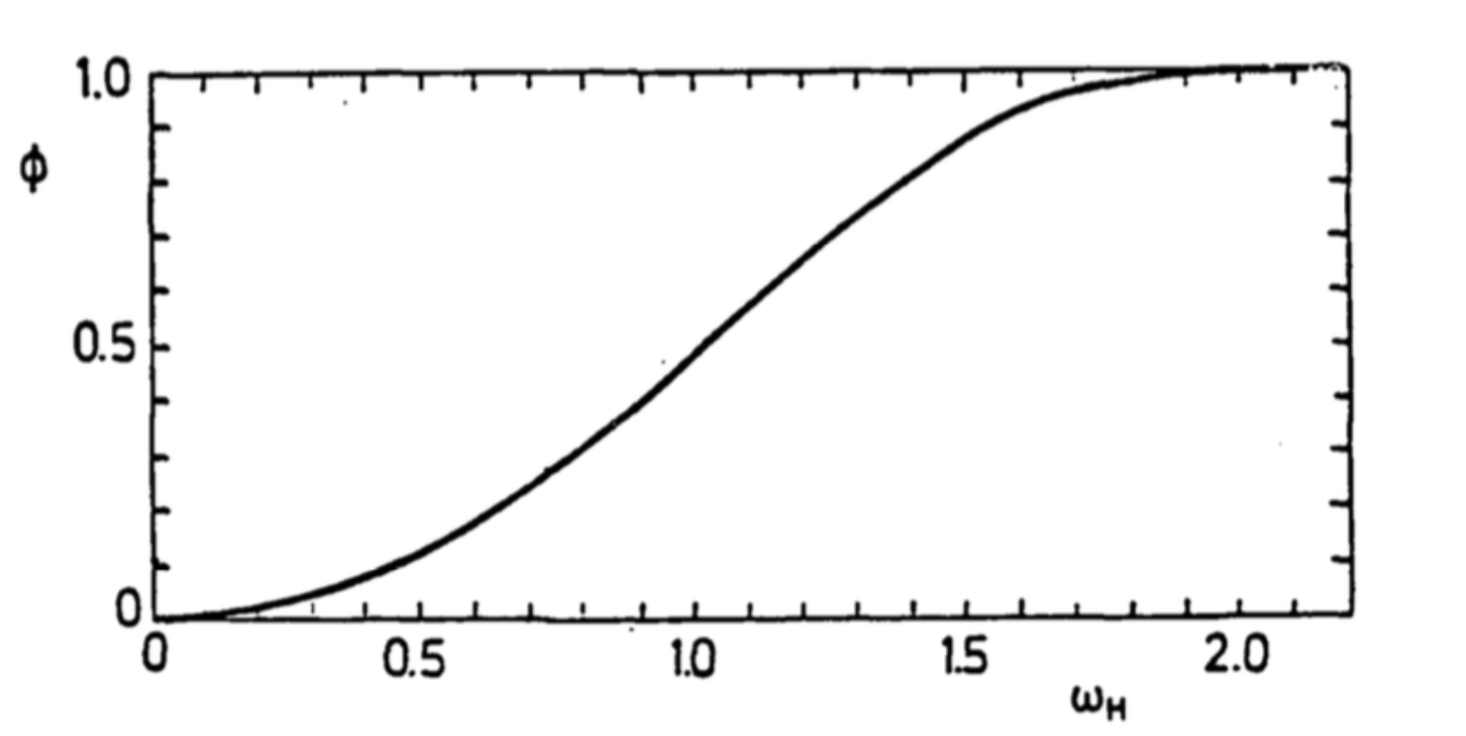
\includegraphics[width=0.45\textwidth]{"images/tma_correction.png"}
    \captionof{figure}{$\Phi(\omega, h)$ as a function of $\omega_h$ \cite{hughes1984}}
    \label{fig:tma_correction}
\end{minipage}

Approximation given by Thomson and Vincent \cite{thompson1983} is:
\begin{equation}
    \begin{aligned}
        &\Phi(\omega, h) \approx
        \begin{cases} 
        \frac{1}{2} \omega_h^{2} & \text{if } \omega_h \leq 1 \\
        1 - \frac{1}{2}(2 - \omega_h)^{2} & \text{if } \omega_h > 1
        \end{cases}
    \end{aligned}
\end{equation}

With $\Phi(\omega, h)$ we can now correct the JONSWAP spectrum for shallow waters:
\begin{equation}
    S_{\text{TMA}}(\omega, h) = S_{\text{JONSWAP}}(\omega) \Phi(\omega, h)
    \label{eq:tma_spectrum}
\end{equation}

\subsubsection{Donelan-Banner Directional Spreading}
Currently, the TMA spectrum cannot be used for our project due to a few issues. Firstly, this spectrum is non-directional, so we need to add directionality to it. Secondly, this spectrum accepts $\omega$ as input, but as we are following J. Tessendorf's \cite{tessendorf2001} paper, we need to use $\mathbf{k}$ as input.
To solve the first problem Horvath Christopher \cite{horvath2015} proposes to use Donelan-Banner Directional Spreading \cite{young1999}:
\begin{equation}
    D(\omega, \theta) = \frac{\beta_s}{2 \tanh(\beta_s\pi)}\text{sech}(\beta_s\theta)^{2}
\end{equation}
where,
$$
\begin{aligned}
    &\beta_s =
    \begin{cases} 
    2.61(\omega/\omega_p)^{1.3} & \text{for } 0.56 < \omega/\omega_p < 0.95 \\
    2.28(\omega/\omega_p)^{-1.3} & \text{for } 0.95 \leq \omega/\omega_p < 1.6 \\
    10^{\epsilon} & \text{for } \omega/\omega_p \geq 1.6
    \end{cases}
\end{aligned}
$$
$$
\epsilon = -0.4 + 0.8393 \cdot e^{-0.567\ln(\omega/\omega_p)^{2}}
$$
$$
\theta = \arctan(k.y / k.x) - \theta_{\text{wind}}
$$

In our project we will use $\omega/\omega_p < 0.95$ for first case as it produces more smooth results.
Now we can combine the TMA spectrum with the Donelan-Banner Directional Spreading:
\begin{equation}
    D_{\text{TMA}}(\omega, \theta) = S_{\text{TMA}}(\omega) \cdot D(\omega, \theta)
\end{equation}

\subsubsection{TMA transformation}
Lastly, to make this spectrum usable, we need to transform it from $\omega$ to $\mathbf{k}$. According to Horvath Christopher \cite{horvath2015}, we can transform it as follows:
\begin{equation}
    S_{\text{TMA}}(\mathbf{k}) = 2S_{\text{TMA}}(\omega, h) \cdot \frac{d\omega}{dk} / k \cdot \Delta k_x \cdot \Delta k_y
    \label{eq:tma_spectrum_k}
\end{equation}
where in our case,
$$
\frac{d\omega}{dk} = \frac{g}{2\sqrt{g*\mathbf{k}}}
$$

\subsection{Cooley-Tukey Fast Fourier Transform (FFT)}
When simulating fourier transform ocean the majority of time is spent on converting from frequency domain to time domain, i.e., performing the IFT.
The previously mentioned IDFT \ref{eq:idft} has time complexity of $O(n^2)$, which is clearly insufficient for simulating higher resolution ocean surfaces in real time.
To address this, the Fast Fourier Transform (FFT) algorithm was invented by Gauss Carl Friedrich in 1805 \cite{gauss1866} and later reinvented by Cooley James W. and Tukey John W. in 1965 \cite{cooley1965}. 
The FFT algorithm, with a time complexity of $O(n\log n)$, exploits the redundancy in the computation of the DFT to reduce the time complexity. It's important to note that the FFT algorithm only works when the number of samples is a power of 2.

The basic idea of the FFT algorithm is as follows:
\begin{enumerate}
    \item Split the input data into two subsets: one containing the even samples and the other containing the odd samples. Repeat this process until each subset contains only 2 samples (this is known as bit-reverse sort order).
    \item Generate twiddle factor $W_N = e^{-i 2 \pi k / N}$ and rise it to the power of \\
    \begin{equation}
        k = i * N / 2^{\text{stage} + 1} \text{ mod } N
    \end{equation}
    where $i$ is the index of the sample, stage is the current stage and $N$ is the number of samples.
    \item Perform butterfly operations \ref{fig:butterfly_diagram}, where $x$ and $y$ are complex numbers and $W$ is the twiddle factor

    \begin{minipage}{1\textwidth}
        \centering
        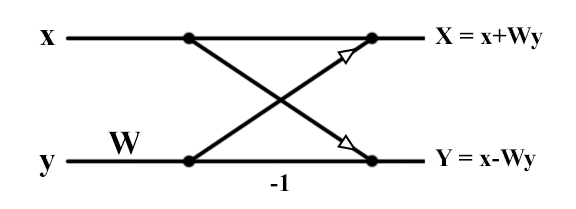
\includegraphics[width=0.4\textwidth]{"images/butterfly_diagram.png"}
        \captionof{figure}{Butterfly Diagram}
        \label{fig:butterfly_diagram}
    \end{minipage}

    \item The butterfly operations are performed in stages \ref{fig:8_butterfly_diagram}. For example, if we have 8 samples, we will have $\log(8) = 3 $ stages. The first stage is for pairs of points (2-point DFTs), the second stage is for groups of four points (4-point DFTs), and so on.
\end{enumerate}

\begin{minipage}{1\textwidth}
    \centering
    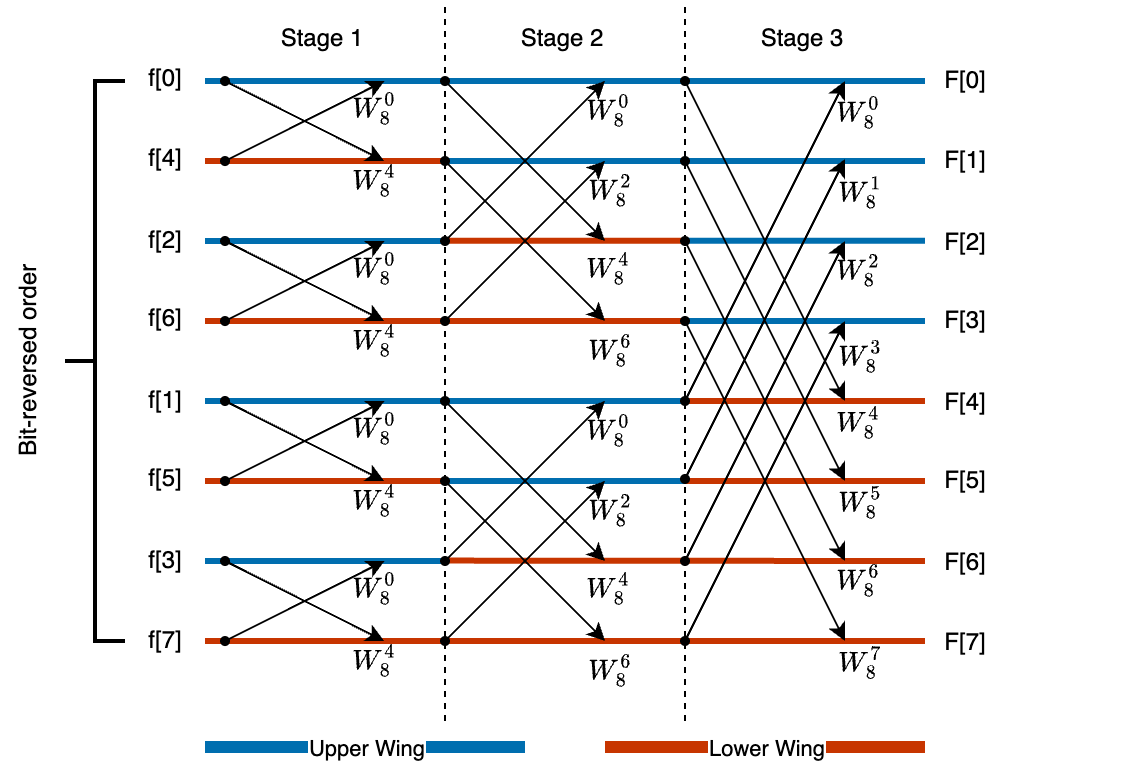
\includegraphics[width=0.7\textwidth]{"images/8_butterfly_diagram.png"}
    \captionof{figure}{8-point FFT Butterfly Diagram}
    \label{fig:8_butterfly_diagram}
\end{minipage}

\subsection{Phong Shading}
The Phong shading model, proposed by Phong Bui Tuong in 1975 \cite{phong1975}, is a simple yet effective method for approximating realistic shading. This model consists of three components: ambient shading, diffuse shading, and specular shading, as shown in Figure \ref{fig:phong_shading}.

\begin{minipage}{1\textwidth}
    \centering
    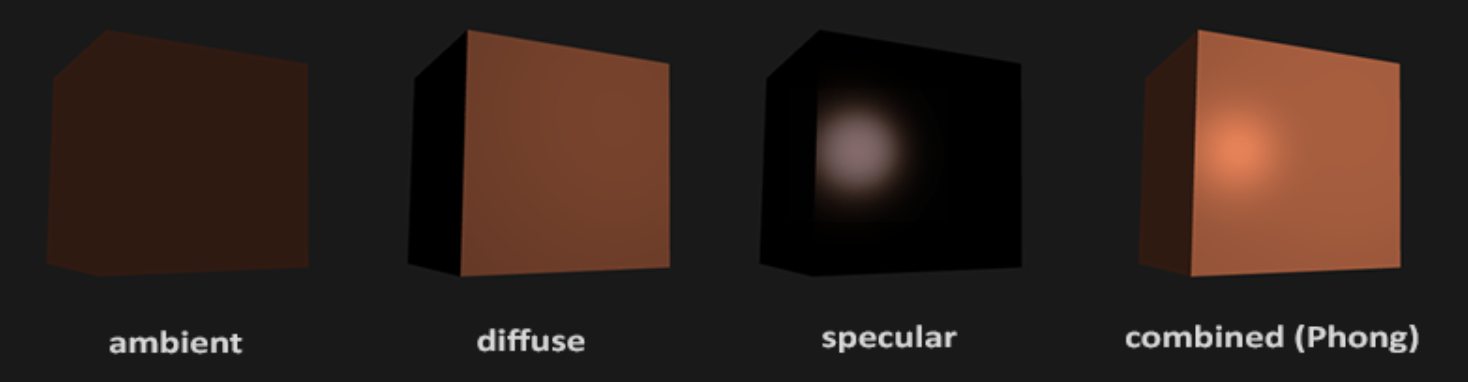
\includegraphics[width=0.6\textwidth]{"images/phong_shading.png"}
    \captionof{figure}{Phong Shading \\ Credits: learnopengl.com}
    \label{fig:phong_shading}
\end{minipage}

The ambient component is a constant value that represents the light scattered throughout the entire scene. The diffuse component can be calculated using the following equation:
\begin{equation}
    \text{Diffuse} = \text{max}(\text{Normal} \cdot \text{LightDirection}, 0.0);
\end{equation}
In this equation, the Normal is a normalized vector that is perpendicular to the surface and points away from it. The specular component can be calculated as follows:
\begin{equation}
    \text{Specular} = max(\text{ViewDir} \cdot \text{ReflectionDir}, 0.0)^{\text{Shininess}}
    \label{eq:phong_specular}
\end{equation}
Here, the ViewDir is a normalized vector pointing towards the camera, and the ReflectionDir is a normalized reflection vector with respect to the Normal. These vectors are illustrated in Figure \ref{fig:phong_graph}.

\begin{minipage}{1\textwidth}
    \centering
    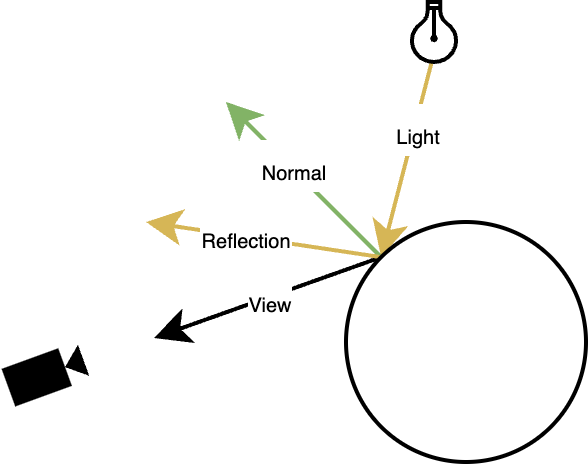
\includegraphics[width=0.4\textwidth]{"images/phong_graph.png"}
    \captionof{figure}{Phong Vectors}
    \label{fig:phong_graph}
\end{minipage}

\subsection{Physically Based Rendering (PBR)}
Earlier mentioned Phong Shading model, does not provide a highly realistic approximation of lighting. To achieve a realistic representation of ocean shading, it is necessary to incorporate a multitude of custom parameters.

Physically Based Rendering (PBR) attempts to address this issue. However, it is important to note that "PBR is more of a conceptual framework than a set of rigid rules" \cite{wilson2017}. The PBR rendering model adheres to three primary principles: energy conservation, microfacet support, and the Fresnel effect.

For the specific application of PBR in ocean shading, one can refer to “Wakes Explosions and Lighting: Interactive Water Simulation in Atlas” by Mark Mihelich and Tim Tcheblokov \cite{mark2021}, which provides an in-depth discussion on the subject. For a more general understanding of PBR, “Physically Based Shading in Theory and Practice” by Stephen Hill and Stephen McAuley \cite{stephan2012} offers comprehensive coverage of the topic from 2012 to 2020.

\subsection{Particle Simulation and Machine Learning}
Particle-based methodologies, known for their ability to simulate water in a realistic and visually compelling manner, are frequently employed in the field of computer graphics. However, these methods come with a high computational cost, which can be a limiting factor.

Recent advancements in Graphics Processing Unit (GPU) technology have started to alleviate this issue. Research, such as that conducted by Libo Huang \cite{huang2021}, is making particle simulations increasingly viable for ocean simulation. However, these techniques still demand a high-performance GPU and are not yet suitable for widespread real-time applications.

In addition to these developments, there have been significant strides in the application of machine learning to accelerate fluid simulations. This is evident in the work of Dmitrii Kochkov \cite{kochkov2021machine}. Despite these advancements, real-time performance on lower-end GPUs remains a challenge.



% Introdunction on my project
% What is ocean simulation
% Why is it important
% What are the applications

% What other people are doing.
% Gersner waves
% FT Ocean
% Diffrent Spectrums
% FFT


% What I do is that is different from others.
% I combined this and this. From there and there.

% Why did I combine these papers and what do I suspect to get out.



\chapter{Methods}
\label{chapter2}

% Have a section for each paper
% Have lot's of graphs and images

% short summary of your method, 1 to 2 paragraphs
% the three sections on the three papers
% implementation details, for example, you can break it down into steps like how you did on reddit
% ps: use as many figure to show your work as possible
% figures include: at least one illustration on how your method work and as many figures on the ocean as possible

\section{Algorithm Overview}
The algorithm can be split into 3 main parts as shown in figure \ref{fig:ocean_algorithm}
\begin{enumerate}
    \item Spectrum generation (Only calculated on parameter value change)
    \item Frequency generation
    \item Convertion from frequency to time domain using IFFT
\end{enumerate}
As shown in figure \ref{fig:ocean_algorithm} majority of calculations are done on GPU using HLSL executed inside Unity. As FFT algorith requires input size to be $2^n$ we going to use 512x512 textures as this provides good performance and high enought details. For simplicity in this project we assume that the texture size is $N$x$N$, where $N$ is the size of a texture and $N$ is power of 2.

\begin{minipage}{1\textwidth}
    \centering
    \includegraphics[width=0.8\textwidth]{"images/ocean_algorithm.png"}
    \captionof{figure}{Ocean Algorithm}
    \label{fig:ocean_algorithm}
\end{minipage}
\section{IFFT}
\subsection{Butterfly Texture \ref{fig:ifft_algorithm}}
Firstlly we only intrested in IFFT algorithm and we will not use FFT.
To perform IFFT we going to produce so called butterfly texture by \cite[Fl{\"u}gge Fynn-Jorin]{flugge2017}.
This texture has width of $(log_2(n)$ and height of $n$ and is precomputed and stored inside the GPU memory once, unless the data size changes. This is 4 chanel texture $(W_r, W_i, y_t, y_b)$,
where $W_r$ and $W_i$ are real and imaginary parts of the twiddle factor, $y_t$ and $y_b$ are top and bottom butterfly indices as shown in \ref{fig:butterfly_diagram}.

In butterfly texture coordinate x represents a stage \ref{fig:8_butterfly_diagram}, while each y represents a butterfly operation between two data points $y_t$ and $y_b$.

In the first stage we assign $y_t$ and $y_b$ in bit reversed order, on the other stages:
\begin{itemize}
    \item If the butterfly wing is top half
    \begin{equation}
        \begin{split}
            y_t &= y_{\text{current}} \\
            y_b &= y_{\text{current}} + 2^{\text{stage}}
        \end{split}
    \end{equation}
    \item If the butterfly wing is bottom half
    \begin{equation}
        \begin{split}
            y_t &= y_{\text{current}} - 2^{\text{stage}} \\
            y_b &= y_{\text{current}}
        \end{split}
    \end{equation}
\end{itemize}
We can determine if the wing is upper or lower half:
\begin{equation}
    \text{wing} = y_{\text{current}} \bmod 2^{(\text{stage} + 1)}
\end{equation}
Lastlly we need to calculate twiddle factors:
\begin{equation}
    \begin{split}
        k &= (y_{\text{current}} \cdot n / 2^{\text{stage} + 1}) \bmod n \\
        W &= \exp(-2\pi i k / n)
    \end{split}
\end{equation}

\subsection{Performing IFFT}
Currentlly our data is stored in 2D texture. While this algorithm only accepts 1D data. Therefore, we need to perform 1D IFFT on each row "horizontally" and then on each column "vertically" \ref{fig:ifft_algorithm}.
By following pseudocode from \cite{flugge2017} we can perform IFFT in 2D:

\begin{lstlisting}[caption={Horizontal Butterfly Operation}, frame=single, numberstyle=\small\color{gray}, captionpos=b]
    float4 butterflyData = ButterflyTexture[float2(Stage, id.x)];
    const float2 twiddle = butterflyData.xy;
    // fetch top butterfly input sample
    topSignal = PingPong0[float2(butterflyData.z, id.y)].xy;
    // fetch bottom butterfly input sample
    bottomSignal = PingPong0[float2(butterflyData.w, id.y)].xy;
    // perform butterfly operation
    h = topSignal + ComplexMult(twiddle, bottomSignal);
\end{lstlisting}

Notice that we are using ping-pong buffers to store intermediate results, as we need to perform multiple IFFT passes, in total $log_2(n)$ passes.
After we perform IFFT on each row, we need to perform for each column:
\begin{lstlisting}[caption={Vertical Butterfly Operation}, frame=single, numberstyle=\small\color{gray}, captionpos=b]
    float4 butterflyData = ButterflyTexture[float2(Stage, id.y)];
    const float2 twiddle = butterflyData.xy;
    // fetch top butterfly input sample
    topSignal = PingPong0[float2(id.x, butterflyData.z)].xy;
    // fetch bottom butterfly input sample
    bottomSignal = PingPong0[float2(id.x, butterflyData.w)].xy;
    // perform butterfly operation
    h = topSignal + ComplexMult(twiddle, bottomSignal);
\end{lstlisting}

\subsection*{Permutation}
Lastlly, our data needs to be permuted as you will see later our data is offseted:
\begin{equation}
    [\text{freq} (-N / 2), \text{ ...}, \text{ freq} (-1), \text{ freq} (0), \text{ freq} (1), \text{ ...}, \text{ freq} (N / 2 - 1)]
\end{equation}
While, our IFFT algorithm expected data to be in the following order:
\begin{equation}
    [\text{freq} (0), \text{ freq} (1), \text{ ...}, \text{ freq}(N - 1)]
\end{equation}
This causes our data to flip sign in grid like pattern therefore we need to permute our data:
\begin{lstlisting}[caption={Data Permutation \cite{flugge2017} }, frame=single, numberstyle=\small\color{gray}, captionpos=b]
    float perms[] = {-1, 1};
    uint index = int((id.x + id.y) % 2);
    float perm = perms[index];
    float h = perm * PingPong1[id.xy].x;
    
    PingPong0[id.xy] = float4(h, h, h, 1);
\end{lstlisting}

\begin{minipage}{1\textwidth}
    \centering
    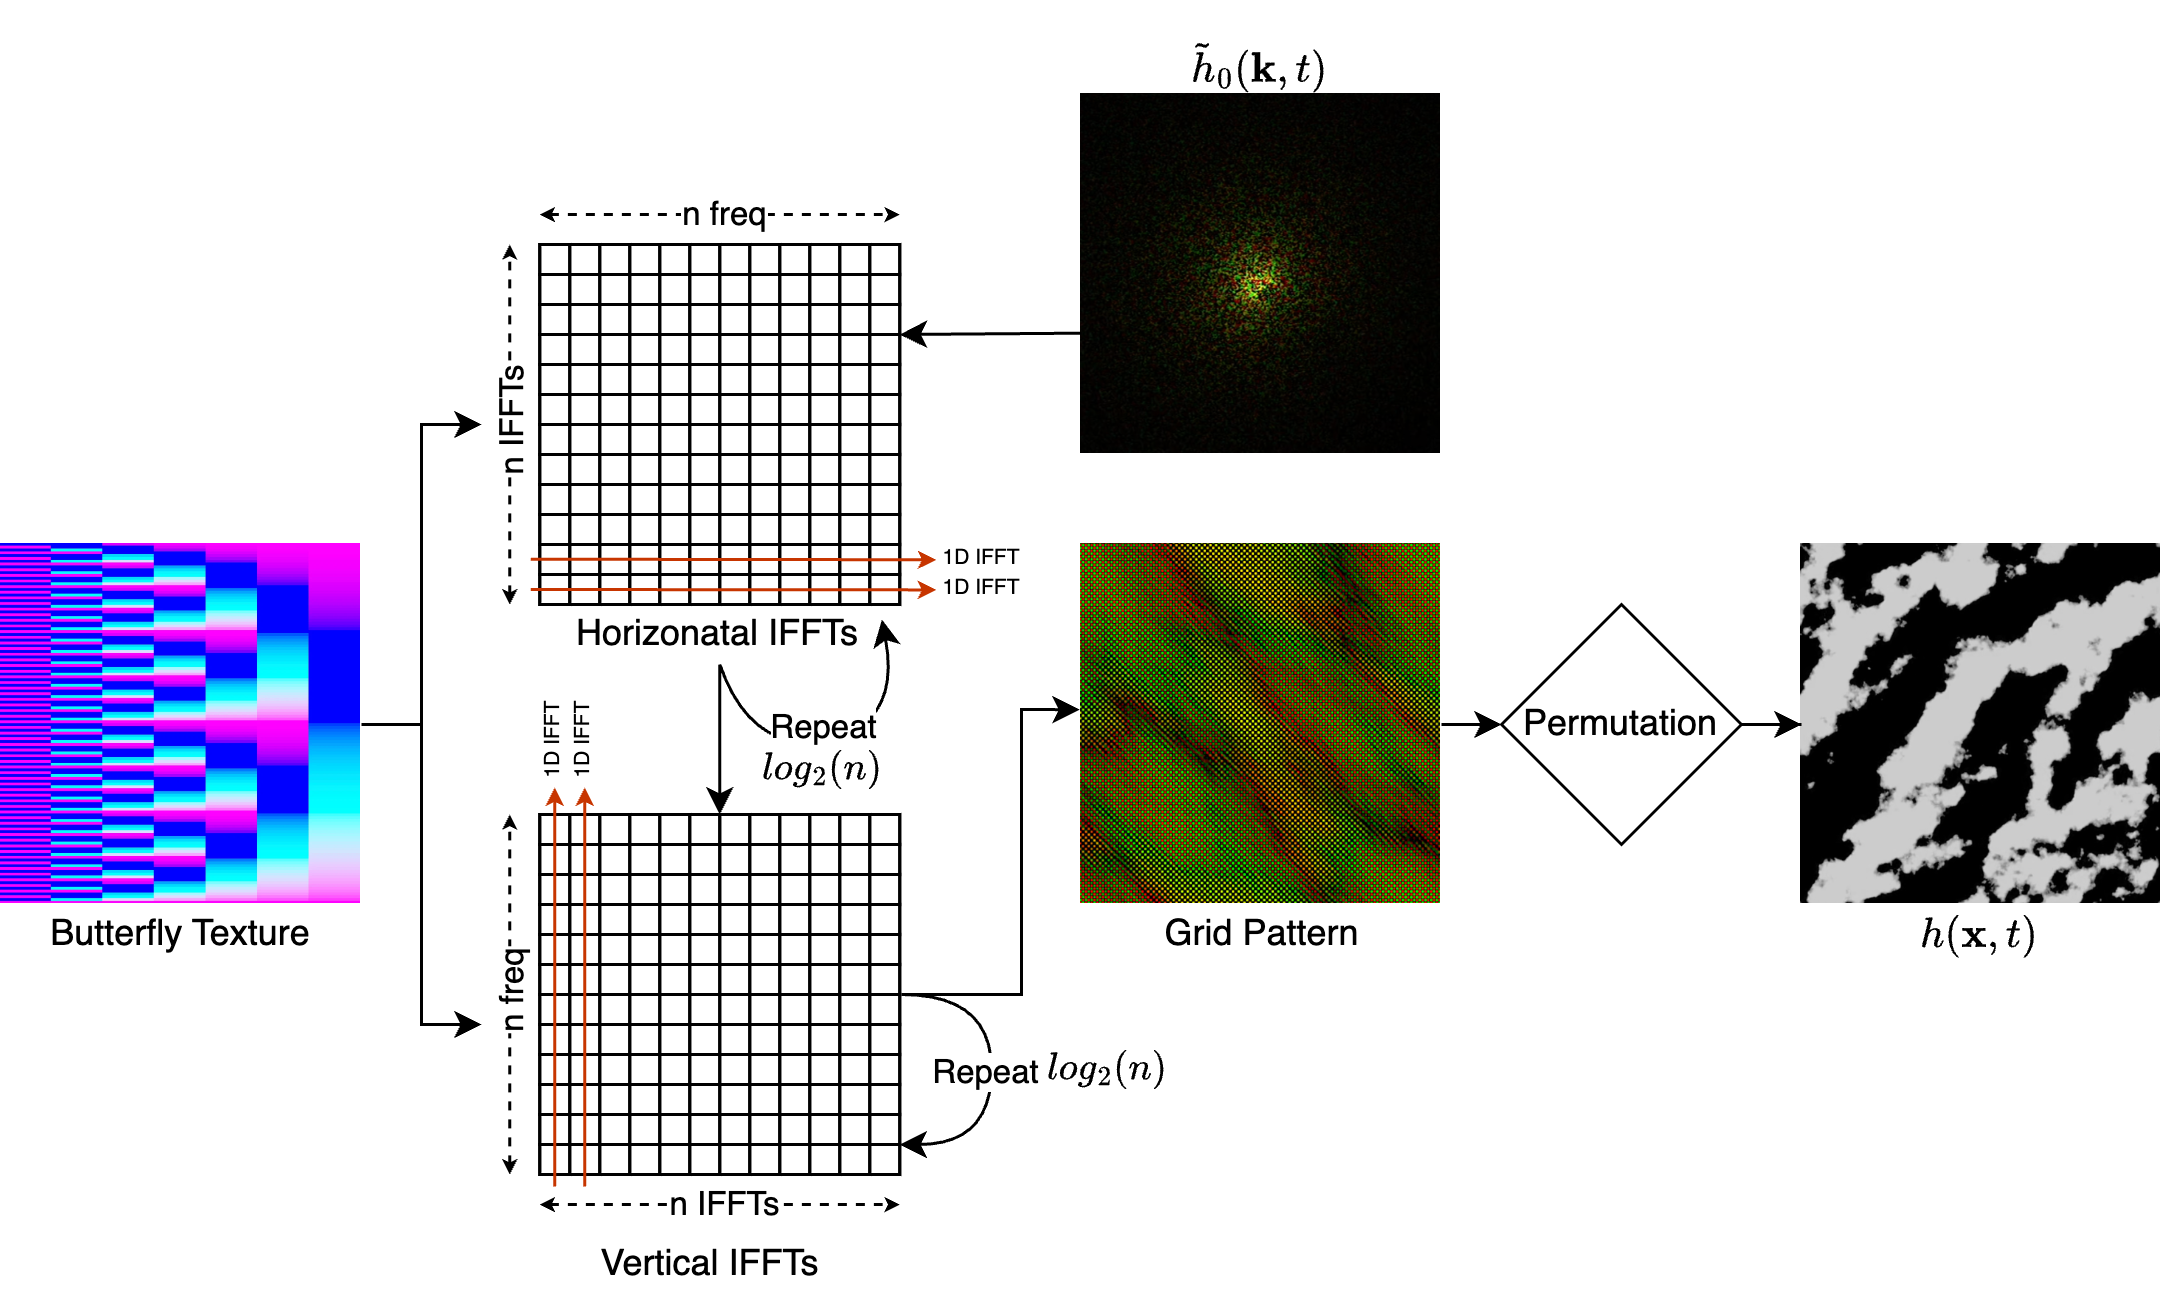
\includegraphics[width=0.7\textwidth]{"images/ifft_algorithm.png"}
    \captionof{figure}{IFFT Algorithm}
    \label{fig:ifft_algorithm}
\end{minipage}

\section{Ocean Geometry}
\subsection{Spectrum Generation}

% Table
\begin{table}[H]
    \centering
    \begin{tabular}{|c|c|}
        \hline
        \textbf{Symbol} & \textbf{Meaning} \\
        \hline
        $S(\omega)$ & Non directional wave spectrum \\
        $S(\omega, \theta)$ & Directional wave spectrum\\
        $S(\mathbf{k})$ & Directional wave spectrum\\
        $\mathbf{k}$ & wave vector \\
        $k$ & Magnetude of wave vector\\
        $l$ & Length scale of the ocean\\
        $\omega$ & dispertion relationship (angular frequency)\\
        $U_{10}$ & Wind speed at 10m above the sea level\\
        $F$ & Fetch (Disntance from lee shore)\\
        $\theta_{\text{wind}}$ & Wind angle\\
        $\lambda$ & Choppy factor\\
        \hline
    \end{tabular}
    \caption{Deffinition Table}
    \label{table:deffinition_table}
\end{table}

Spectrums are responsable for whole look of the ocean. It's importatnt to pick the one that is based on real world data to make our ocean look realistic.
Initialy, Tessendorf spectrum \ref{eq:tessendorf_spectrum} was implemented as it was straight forward to implement. However, it didn't produce satisfying results, as waves didn't seem to transfer energy in convincing way, waves didn't seem to follow wave direction and it was hard to have artistic control over the ocean.

\begin{minipage}{1\textwidth}
    \centering
    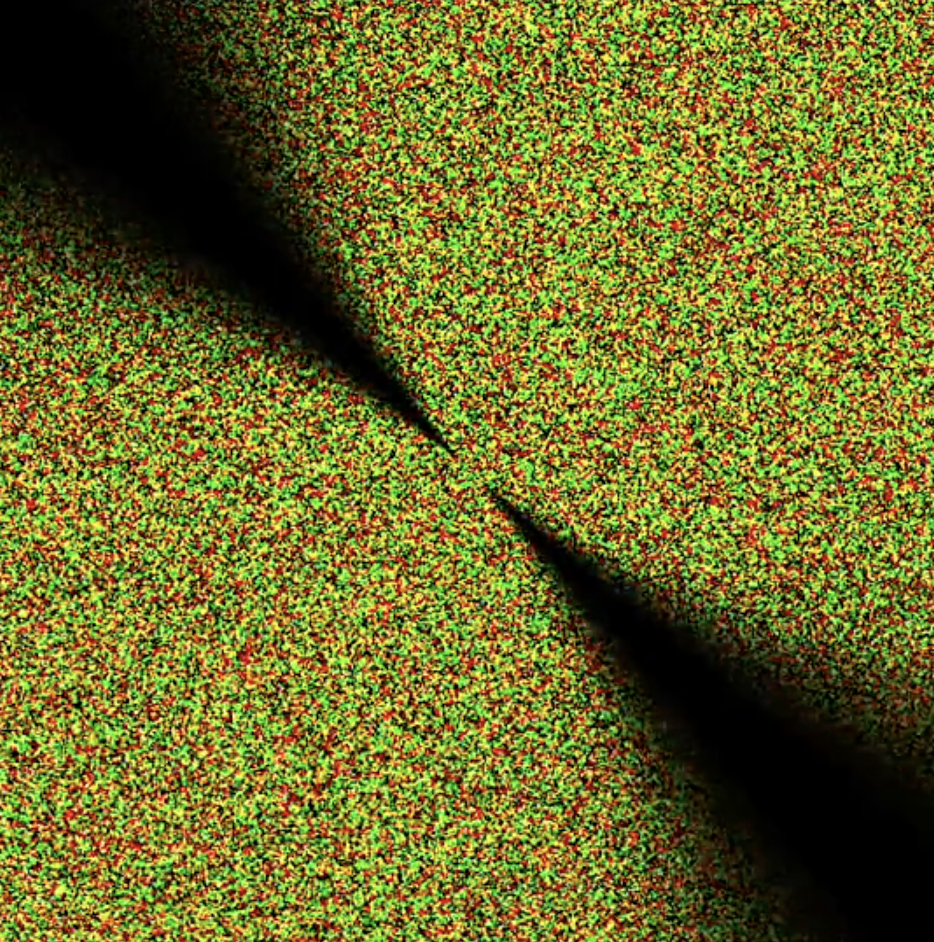
\includegraphics[width=0.4\textwidth]{"images/phillips_spectrum.png"}
    \captionof{figure}{Jerry Tessendorf's Spectrum}
    \label{fig:phillips_spectrum}
\end{minipage}

Therefore, TMA spectrum \ref{eq:tma_spectrum_k} was implemented.

$$
    S_{\text{TMA}}(\mathbf{k}) = 2S_{\text{TMA}}(\omega, h) \cdot \frac{d\omega}{dk} / k \cdot \Delta k_x \cdot \Delta k_y
$$
where $\mathbf{k} = (k_x, k_y)$, $k_x = 2 * \pi (x_x - n/2)/ l$, $k_y = 2 * \pi (x_y - n/2)/ l$, $l$ is the the length scale of the ocean, 
and $\mathbf{x} = (x_x, x_y)$ is current position in the texture. 

This spectrum resulted in more relistic looking ocean with intuitive controls: fetch, wind speed, wind angle, depth. Moreover, it didn't require any efort to make the ocean look relistic and it just worked out of the box.
\begin{minipage}{1\textwidth}
    \centering
    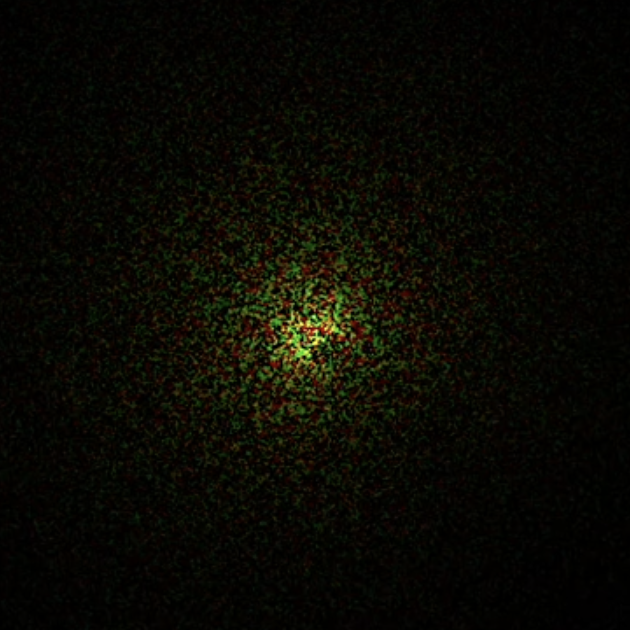
\includegraphics[width=0.40\textwidth]{"images/tma_spectrum.png"}
    \captionof{figure}{TMA spectrum, Frequency Domain \\ (100x for better visibility)}
    \label{fig:tma_spectrum}
\end{minipage}

\subsection{Height Map Generation}

To generate height map, firstlly we need to have fourier amplitudes as shown in \ref{eq:fouier_amplitudes}, where $P_h$ is TMA Spectrum $S_{TMA}(\mathbf{k})$.
For the next step we need to add fourier amplitude and it's complex conjugate to produce "produce waves towards and against the wave direction when propagating"\cite{horvath2015}.
In our luck we don't need to recalculate complex conjugate as fourier series are symetric, so we can just mirror the amplitudes:
\begin{equation}
    \tilde{h}^{*}_0 = T_{h_0}(x^{*}, y^{*})
\end{equation}
where $T_{h_0}(x, y)$ is fourier amplitude in precomputed texture at $x^{*} = (n - x) \text{ mod } n$, $y^{*} = (n - y) \text{ mod } n$, $(x, y)$ is current position in the texture.

By having combined amplitudes \ref{eq:combined_amplitudes} we can perform IFFT as shown in \ref{fig:ifft_algorithm} to produce height map.
\begin{minipage}{1\textwidth}
    \centering
    
\includegraphics[width=0.40\textwidth]{"images/tma_height.png"}
    \captionof{figure}{Height Map using $S_{\text{TMA}}$}
    \label{fig:tma_height_map}
\end{minipage}

\subsection{Normal Map Generation}
Latter we will need extra information about the ocean to calculate ocean shading. Therefore, we need to calculate normal map. Normal map is perpendicular direction to the surface of the ocean.
To calculate normal map we need to calculate gradient, which is derivative of the height map. According to \cite{tessendorf2004} the derivative is:
\begin{equation}
    \epsilon(\textbf{x}, t) = i\textbf{k} \tilde{h}(\textbf{k}, t)
\end{equation}
Then we need to perform IFFT \ref{fig:ifft_algorithm} to get normal map in the time domain.

\begin{minipage}{1\textwidth}
    \centering
    
\includegraphics[width=0.40\textwidth]{"images/tma_normal.png"}
    \captionof{figure}{Normal Map using $S_{\text{TMA}}$}
    \label{fig:tma_normal_map}
\end{minipage}

\subsection{Choppy Waves}
Currentlly, when rendering ocean it looks too smooth \ref{fig:ocean_no_choppy} and lacks choppiness.

\begin{minipage}{1\textwidth}
    \centering
    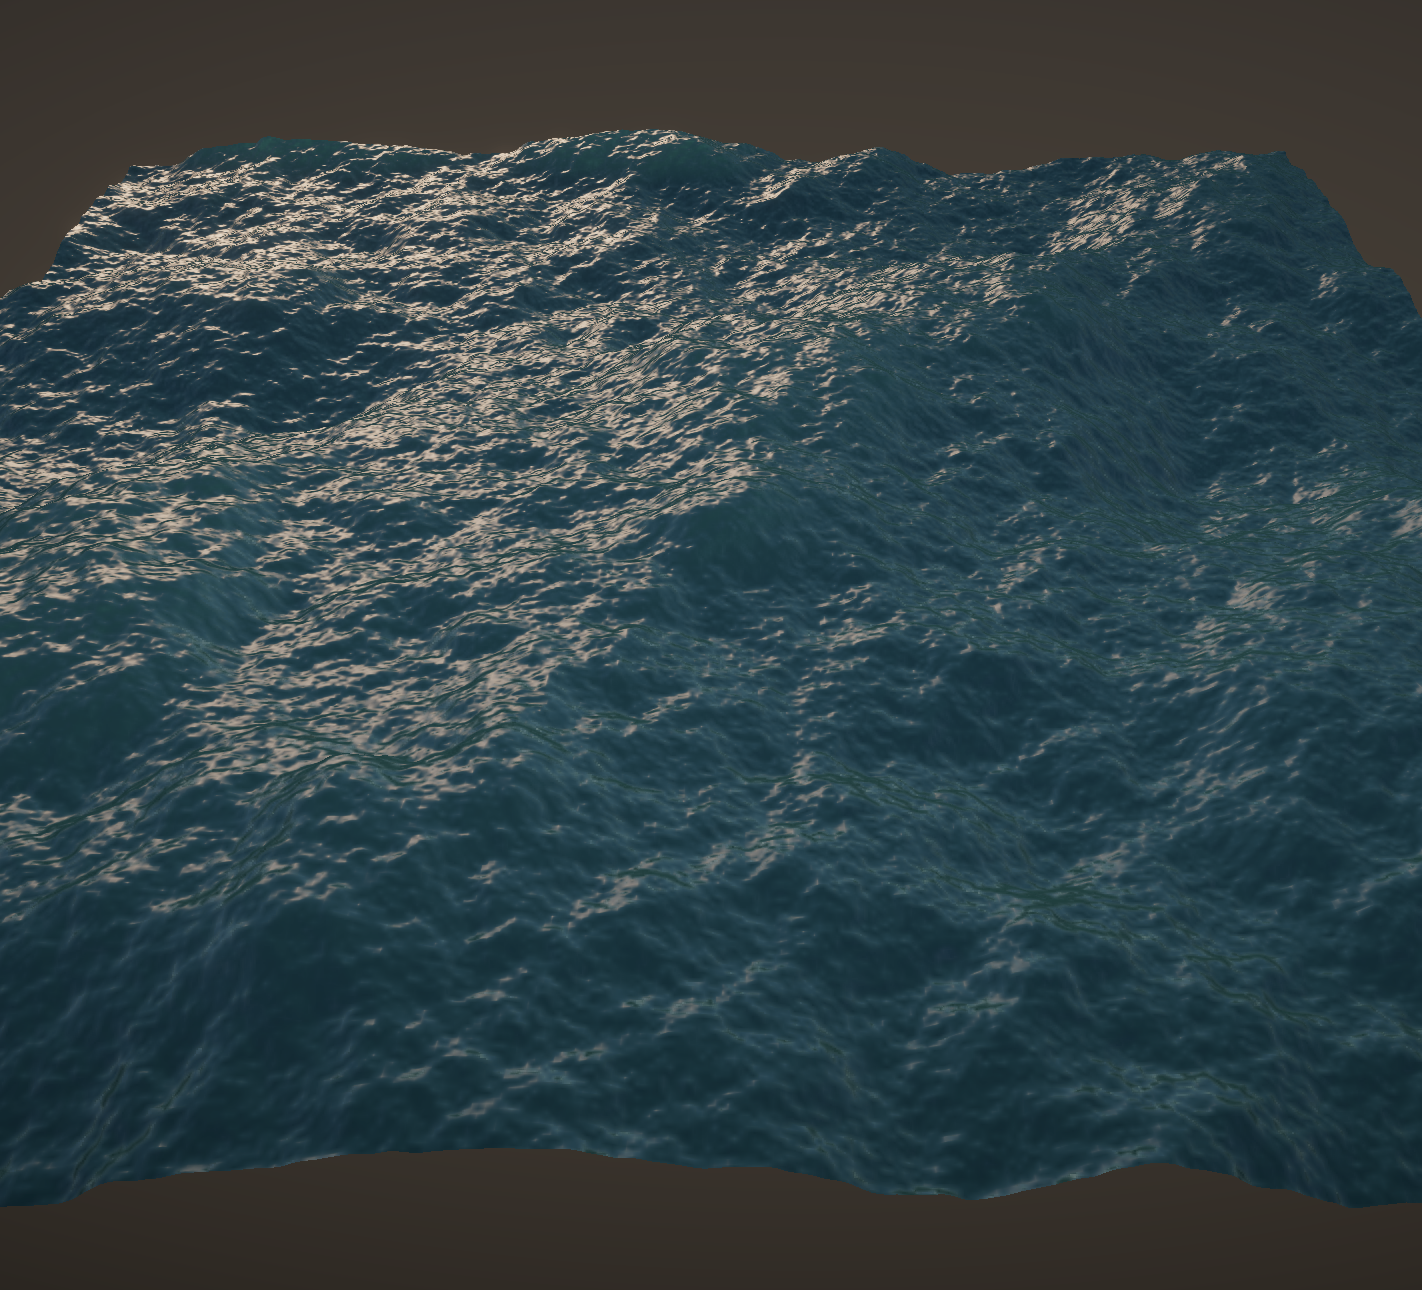
\includegraphics[width=0.40\textwidth]{"images/rendered_height_no_coppy.png"}
    \captionof{figure}{Ocean without Choppy Waves}
    \label{fig:ocean_no_choppy}
\end{minipage}

To make waves choppy we need to introduce horizotal displacement. This will not only make waves more chopy but also make energy transfer between waves more relistic. Following formula from \cite[J. Tessendorf]{tessendorf2004} we can calculate horizontal displacement:
\begin{equation}
    \mathbf{D}_{\text{hori}}(\textbf{x}, t) = -i\frac{\mathbf{k}}{k}\tilde{h(\mathbf{k}, t)}
\end{equation}
Using this horizotal displacement we can displace our verticies:
\begin{equation}
    \mathbf{x} + \lambda \mathbf{D}_{\text{hori}}(\textbf{x}, t)
\end{equation}
, where $\lambda$ is "choppy factor".
Once again we need to perform IFFT \ref{fig:ifft_algorithm} to get horizontal displacement in the time domain.

\begin{minipage}{1\textwidth}
    \centering
    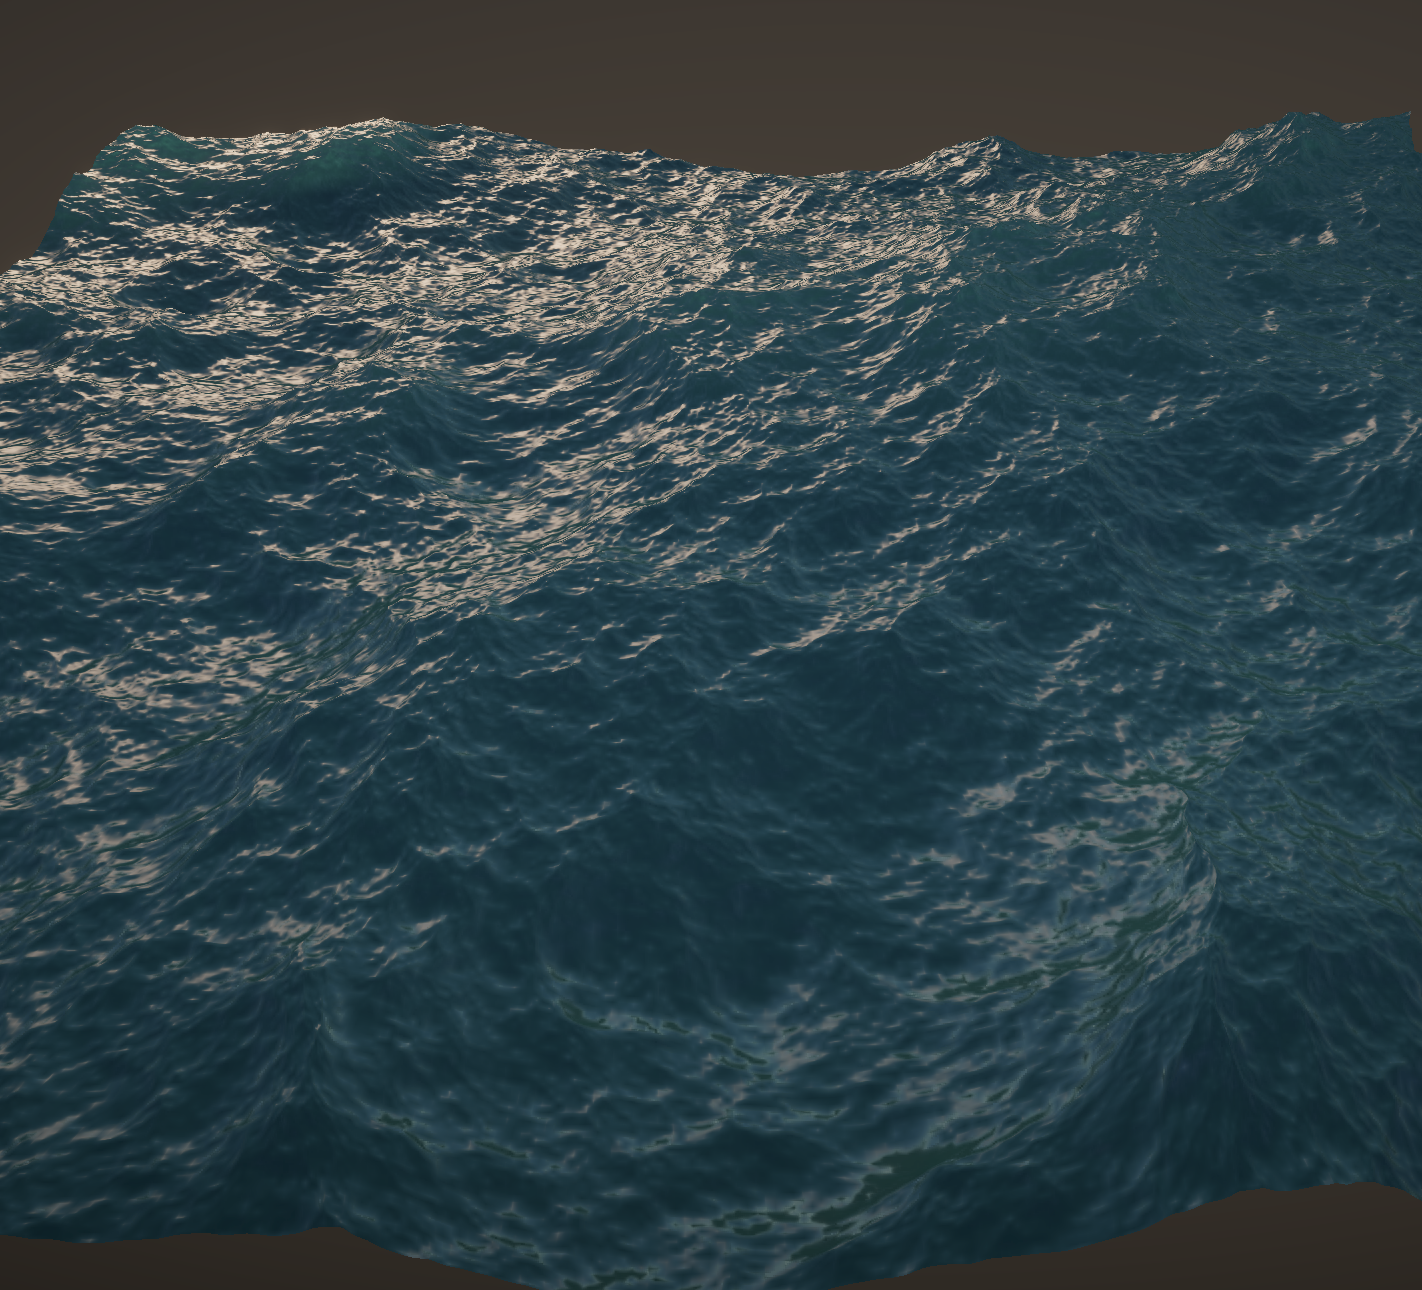
\includegraphics[width=0.40\textwidth]{"images/rendered_height_choppy.png"}
    \captionof{figure}{Ocean with Choppy Waves}
    \label{fig:ocean_choppy}
\end{minipage}

\section{Ocean Shading}

\begin{table}[H]
    \centering
    \begin{tabular}{|c|c|c|}
        \hline
        \textbf{Symbol} & \textbf{Parameter} \\
        \hline
        $L_a$ & Ambient Light \\
        $L_ss$ & Subsurface Scatter Light\\
        $L_s$ & Specular Light\\
        $L_r$ & Enviroment Reflection\\
        $N$ & Normal \\
        $D_s$ & Sun Direction \\
        $D_v$ & View Direction \\
        $C_a$ & Ambient Light Color \\
        $C_l$ & Light Color \\
        $C_b$ & Air Bubble Color \\
        $C_{ws}$ & Water Scattering Color \\
        $H$ & Ocean Height \\
        $F$ & Fresnel Effect \\
        $\rho_a$ & Air Bubble Density \\
        $k_a$ & Ambient Light Intensity \\
        $k_{ss_1}$ & Subsurface Scattering Intensity \\
        $k_{ss_2}$ & Subsurface Scattering Intensity \\
        \hline
    \end{tabular}
    \caption{Lighting Parameters}
    \label{table:lighting_parameters}
\end{table}

\subsection{Lighting Model}

\subsubsection{Output}
For our lighting model we going to have 4 components as shown in \ref{eq:light_model}. These components are 
ambient light, subsurface scattering, specular light and enviroement reflection. The final output should look like as shown in figure \ref{fig:output_light}
\begin{equation}
    L = L_a + L_{ss} + L_s + L_r
    \label{eq:light_model}
\end{equation}
\begin{minipage}{1\textwidth}
    \centering
    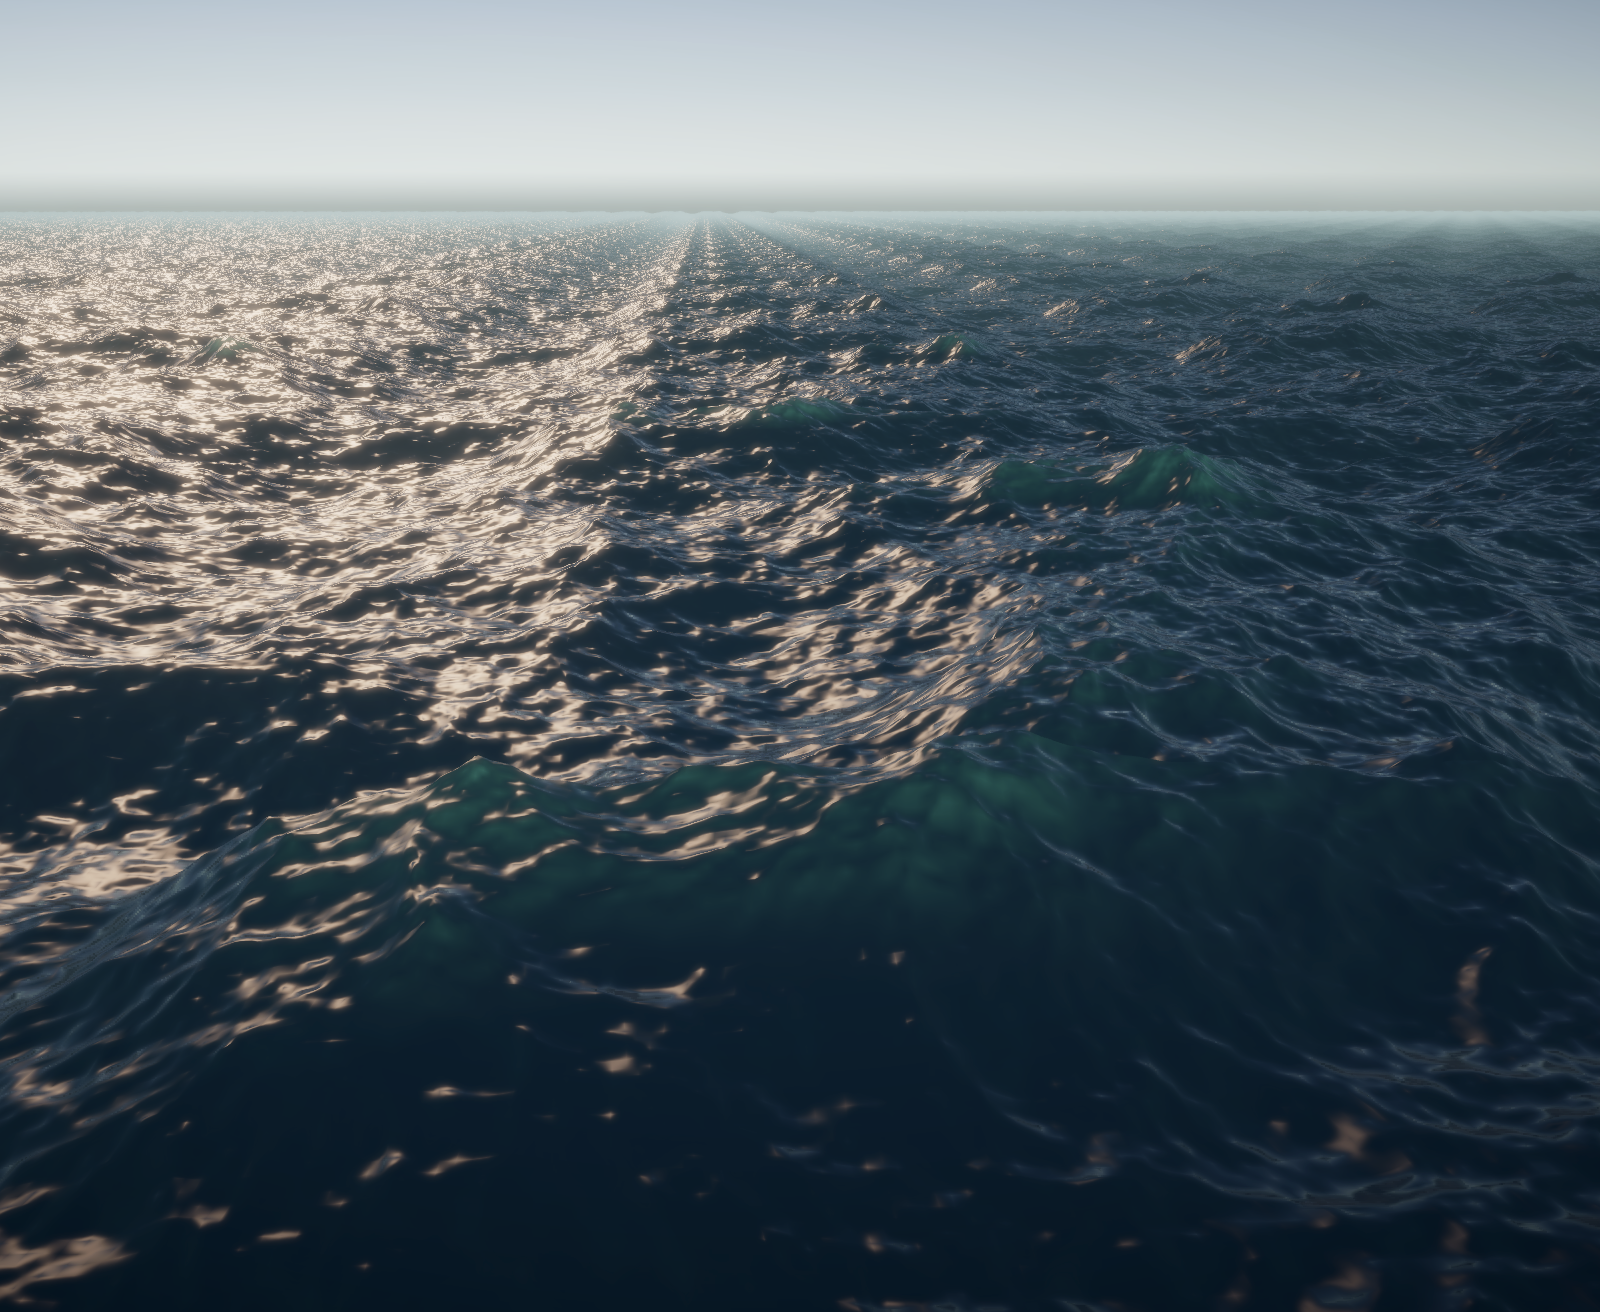
\includegraphics[width=0.50\textwidth]{"images/output_light.png"}
    \captionof{figure}{Finall Shader Output}
    \label{fig:output_light}
\end{minipage}

\subsubsection{Ambient Light}
Ambient light is light that does not come from any specific light source, but rather result of light being scattered in the environment. It is constant and does not depend on the direction of the light source.
For ocean we use  ambient light aproximation formula taken from GDC confference \cite{mark2021}:
\begin{equation}
    L_a = k_a N C_a C_l + \rho_a C_b C_l
\end{equation}
\begin{minipage}{1\textwidth}
    \centering
    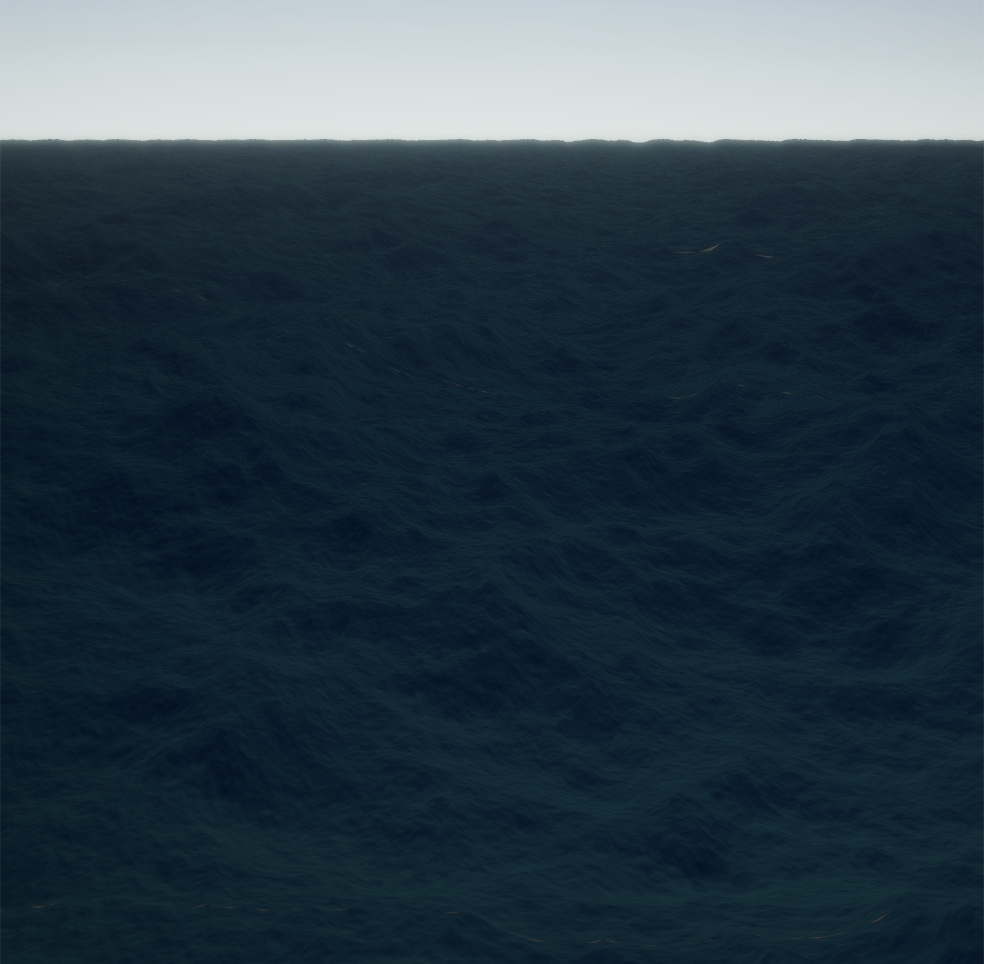
\includegraphics[width=0.40\textwidth]{"images/ambient_light.png"}
    \captionof{figure}{Ambient Light}
    \label{fig:ambient_light}
\end{minipage}

\subsubsection{Fresnel Effect}
Fresnel effect is the phenomenon where light is more reflective at grazing angles. This effect will be importatnt for specular and reflection calculations.
\begin{equation}
    F = (1 - \max(D_v \cdot N, 0.15))^{5}
\end{equation}
\begin{minipage}{1\textwidth}
    \centering
    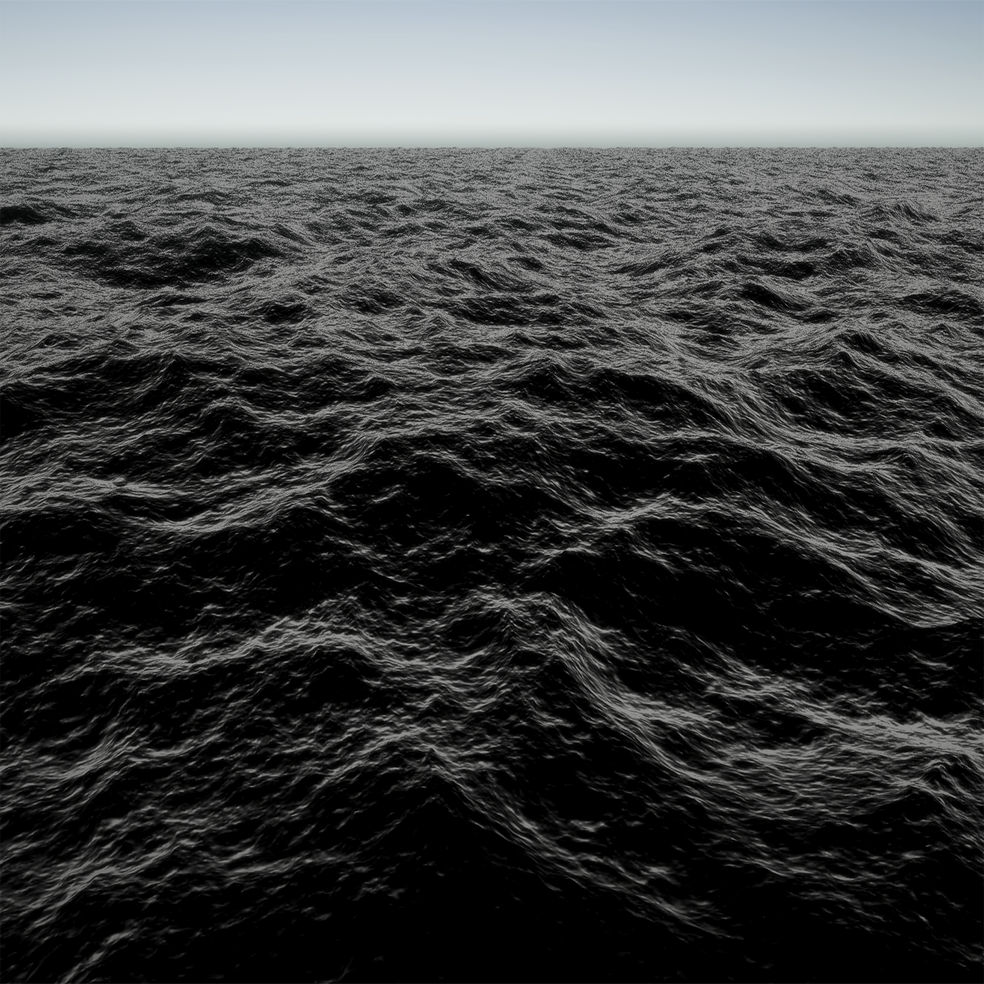
\includegraphics[width=0.45\textwidth]{"images/fresnel.png"}
    \captionof{figure}{Fresnel Effect}
    \label{fig:fresnel_effect}
\end{minipage}

\subsubsection{Subsurface Scattering}
Subsurface scattering is behaviour how light interacts when entering object. In this case how water acts when enttering water body.
Tipacally we would need to have raytracing for relistic results. Fortunetlly, most of our light is trapped in the ocean and only light in wave peeks can escape. 
We can use the approximation from from GDC confference \cite{mark2021}.
\begin{equation}
    \begin{split}
        L_{ss} &= (L_{ss_1} + L_{ss_2}) C_{ws} C_l\\
        L_{ss_1} &= k_{ss_1} \max(0, H) ([D_s, -D_v])^{4}(0.5-0.5(D_s \cdot N))^{3}\\
        L_{ss_2} &= k_{ss_2} ([D_V, N])^{2}
    \end{split}
\end{equation}
\begin{minipage}{0.32\textwidth}
    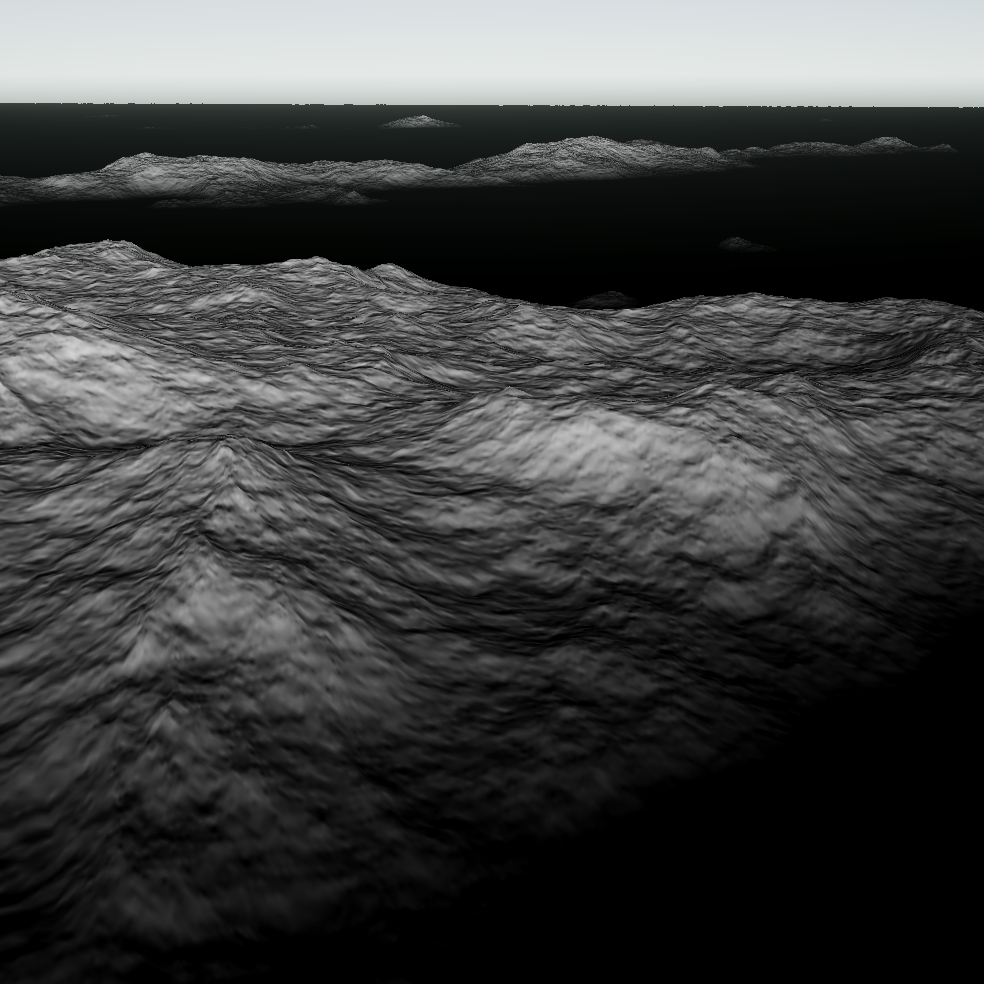
\includegraphics[width=1\textwidth]{"images/ss1_light.png"}
    \captionof{figure}{$L_{ss_1}$}
    \label{fig:lss1_light}
\end{minipage}
\hfill
\begin{minipage}{0.32\textwidth}
    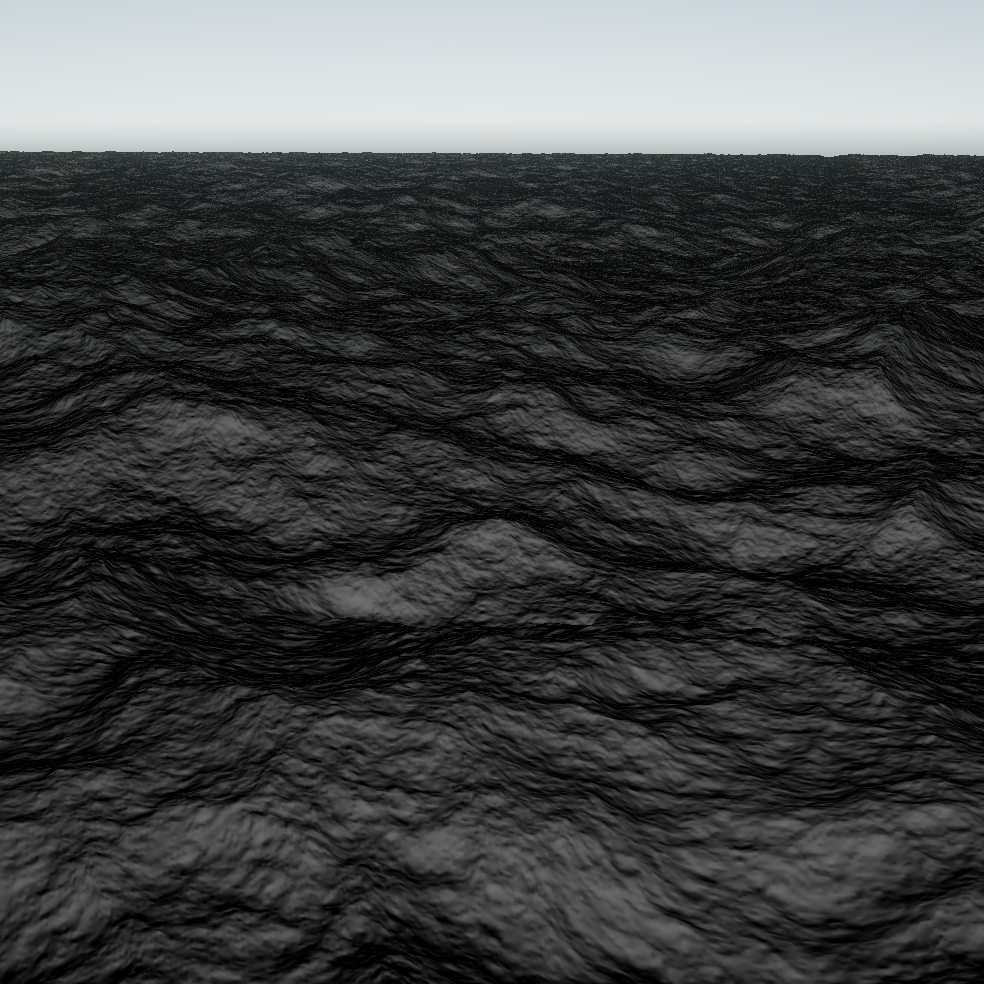
\includegraphics[width=1\textwidth]{"images/ss2_light.png"}
    \captionof{figure}{$L_{ss_2}$}
    \label{fig:lss2_light}
\end{minipage}
\hfill
\begin{minipage}{0.32\textwidth}
    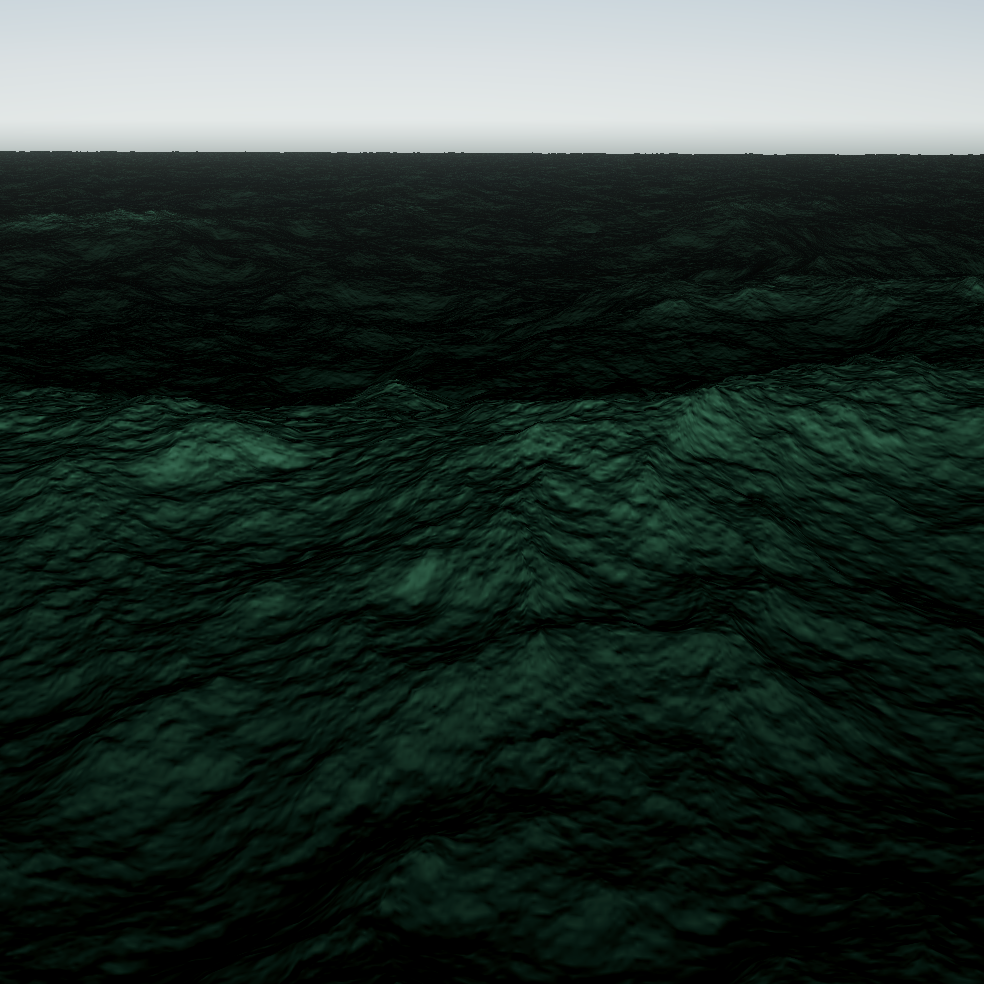
\includegraphics[width=1\textwidth]{"images/ss_light.png"}
    \captionof{figure}{Subsurface Scattering}
    \vspace*{-13pt}
    \label{fig:lss_light}
\end{minipage}

\subsubsection{Specular Reflection}
Specular reflection is a light source reflection on the object that we see on the shiny objects like metals or plastic.
We are using simple phong scatter technique as shown in figure \ref{fig:specular_light} and the formula takes form:
\begin{equation}
    \begin{split}
        L_s &= C_l S C_s F\\
        S &= [D_v, D_r]^{\text{Shininess}}\\
        D_r &= \text{reflect}(\text{LightPos}, N)
    \end{split}
\end{equation}
\begin{minipage}{1\textwidth}
    \centering
    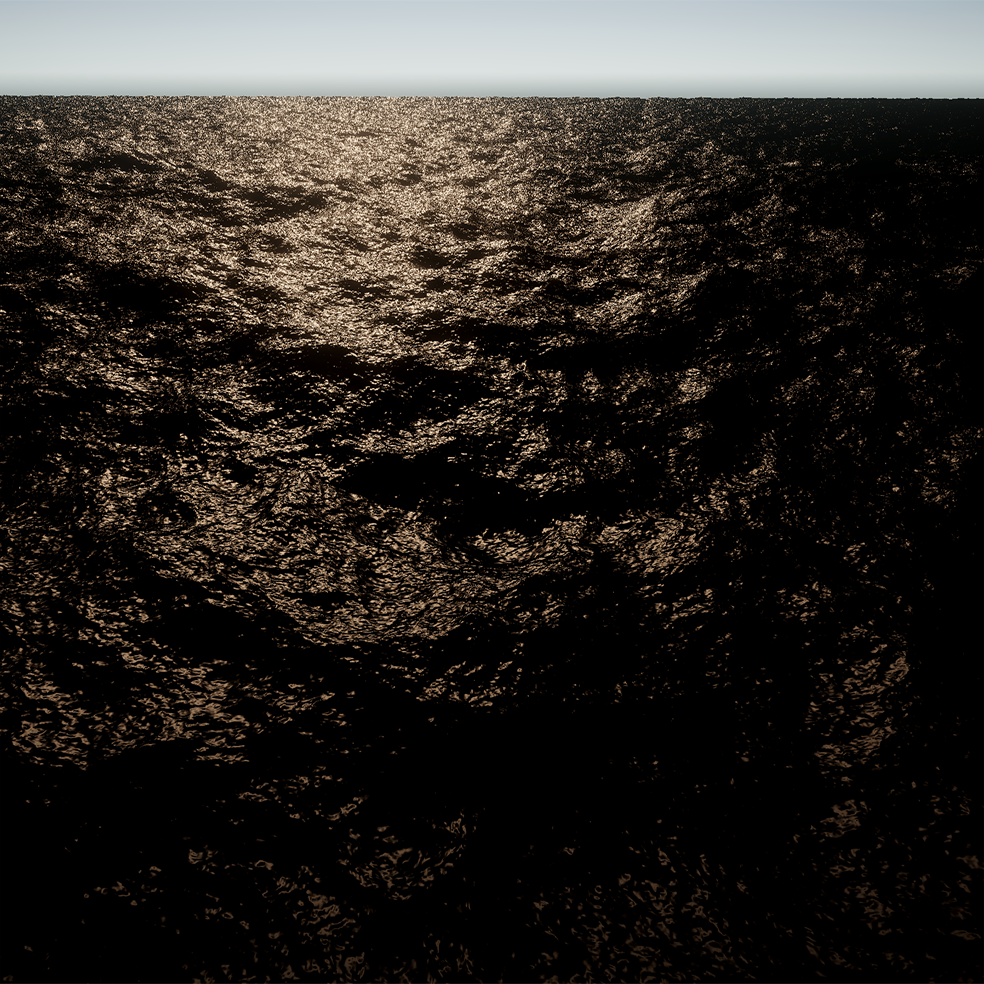
\includegraphics[width=0.45\textwidth]{"images/specular_light.png"}
    \captionof{figure}{Specular Reflection}
    \label{fig:specular_light}
\end{minipage}

\subsubsection{Enviroment Reflection}
For our project we only going to consider skybox reflection on water surface. As per figure \ref{fig:relfection_light} we show how skybox reflection works on calm ocean surface to better visualise enviroment reflection. 
\begin{equation}
    \begin{split}
        L_r &= F k_r C_{\text{sky}}\\
        C_{\text{sky}} &= \text{Sky}[\text{reflect}{D_i, N}]
    \end{split}
\end{equation}
\begin{minipage}{1\textwidth}
    \centering
    
\includegraphics[width=0.45\textwidth]{"images/reflection_light.png"}
    \captionof{figure}{Skybox reflection on calm ocean}
    \label{fig:relfection_light}
\end{minipage}

\subsection{Foam}
\subsubsection{Foam Generation}
\begin{minipage}{1\textwidth}
    \centering
    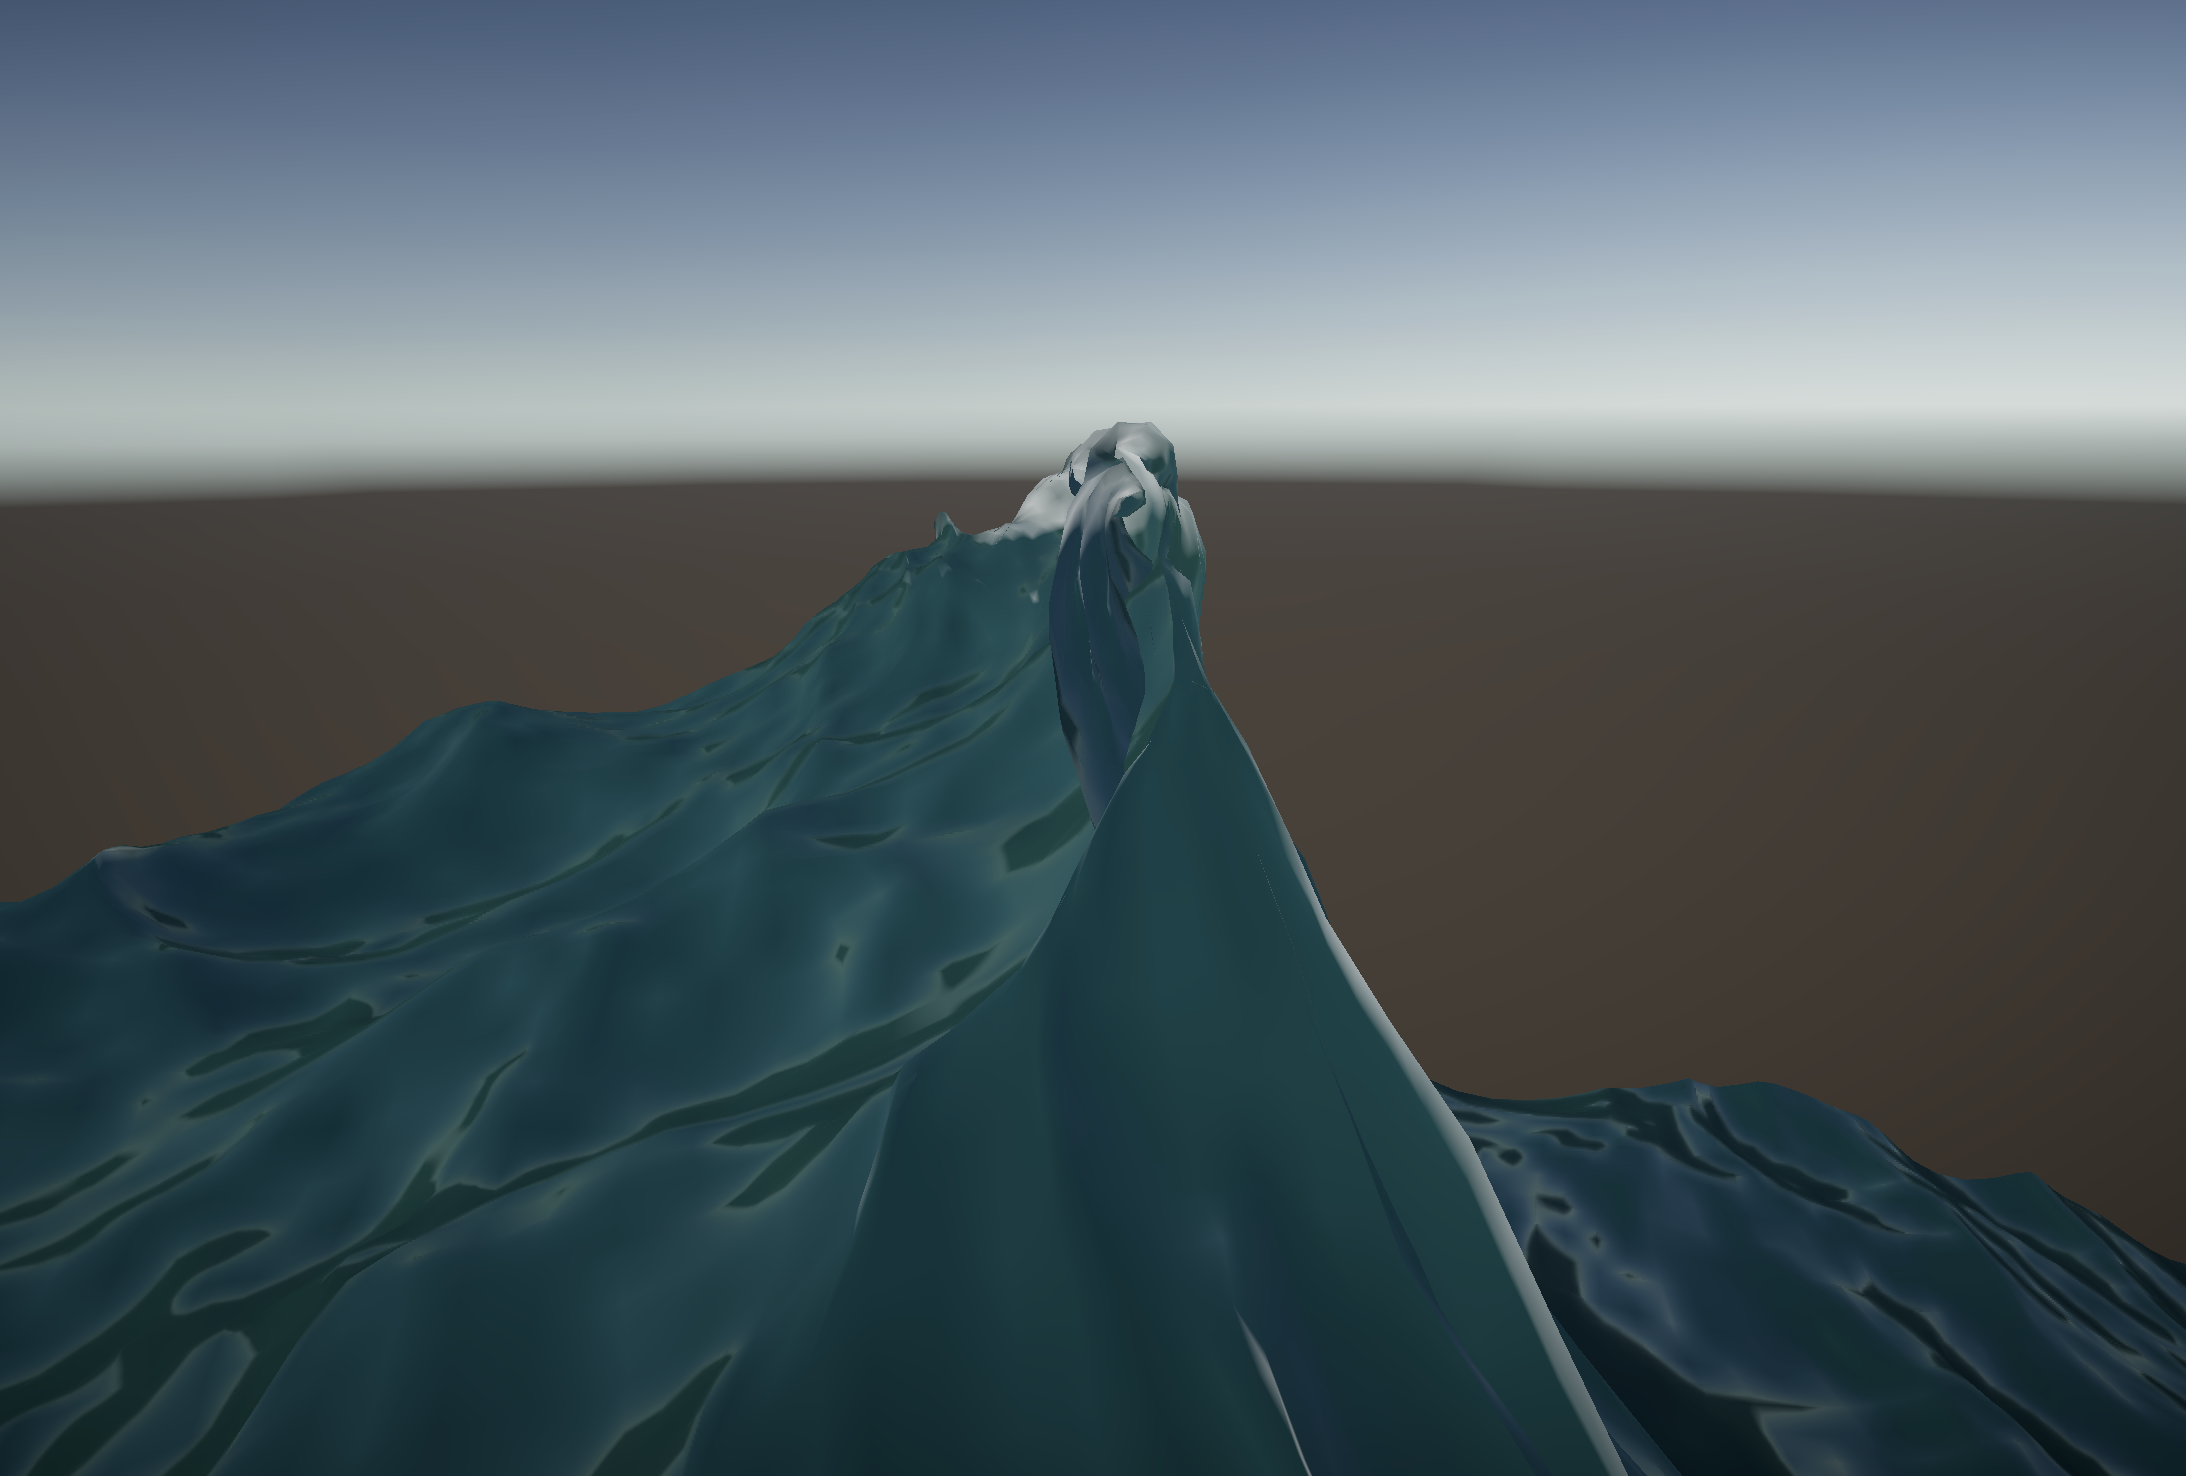
\includegraphics[width=0.50\textwidth]{"images/wave_curl.png"}
    \captionof{figure}{Wave Curl At Wave Peek}
    \label{fig:wave_curl}
\end{minipage}

Ocean foam is a salient and realistic feature of the ocean, contributing to its distinct and authentic appearance. The primary occurrence of foam is observed during wave crashes, a phenomenon facilitated by horizontal displacement. This can be visually discerned at the peaks of waves where the water curls up, as illustrated in Figure \ref{fig:wave_curl}. In essence, our horizontal transformation undergoes an inversion.

As proposed by Tessendorf \cite{tessendorf2001}, the rendering of foam can be achieved by calculating the determinant of the Jacobian matrix for horizontal displacement, which helps identify these inversions. In our ocean simulation, the Jacobian matrix provides insights into the changes over the x and z axes. When determinant of the Jacobian matrix is bellow zero the "wave crash" happens:

\begin{equation}
    \text{Det}(\mathbf{x}) = J_{xx} + J_{yy} - J_{xy} J_{yx}
\end{equation}
where,
\begin{equation}
    J(\mathbf{x}) = 
    \begin{bmatrix} 
        1 + \lambda\frac{\partial D_x(\mathbf{x})}{\partial x} & 1 + \lambda\frac{\partial D_x(\mathbf{x})}{\partial y} \\
        1 + \lambda\frac{\partial D_y(\mathbf{x})}{\partial x} & 1 + \lambda\frac{\partial D_y(\mathbf{x})}{\partial y} 
    \end{bmatrix} 
\end{equation}
in this case $J_{xy} = J_{yx}$.

\begin{minipage}{1\textwidth}
    \centering
    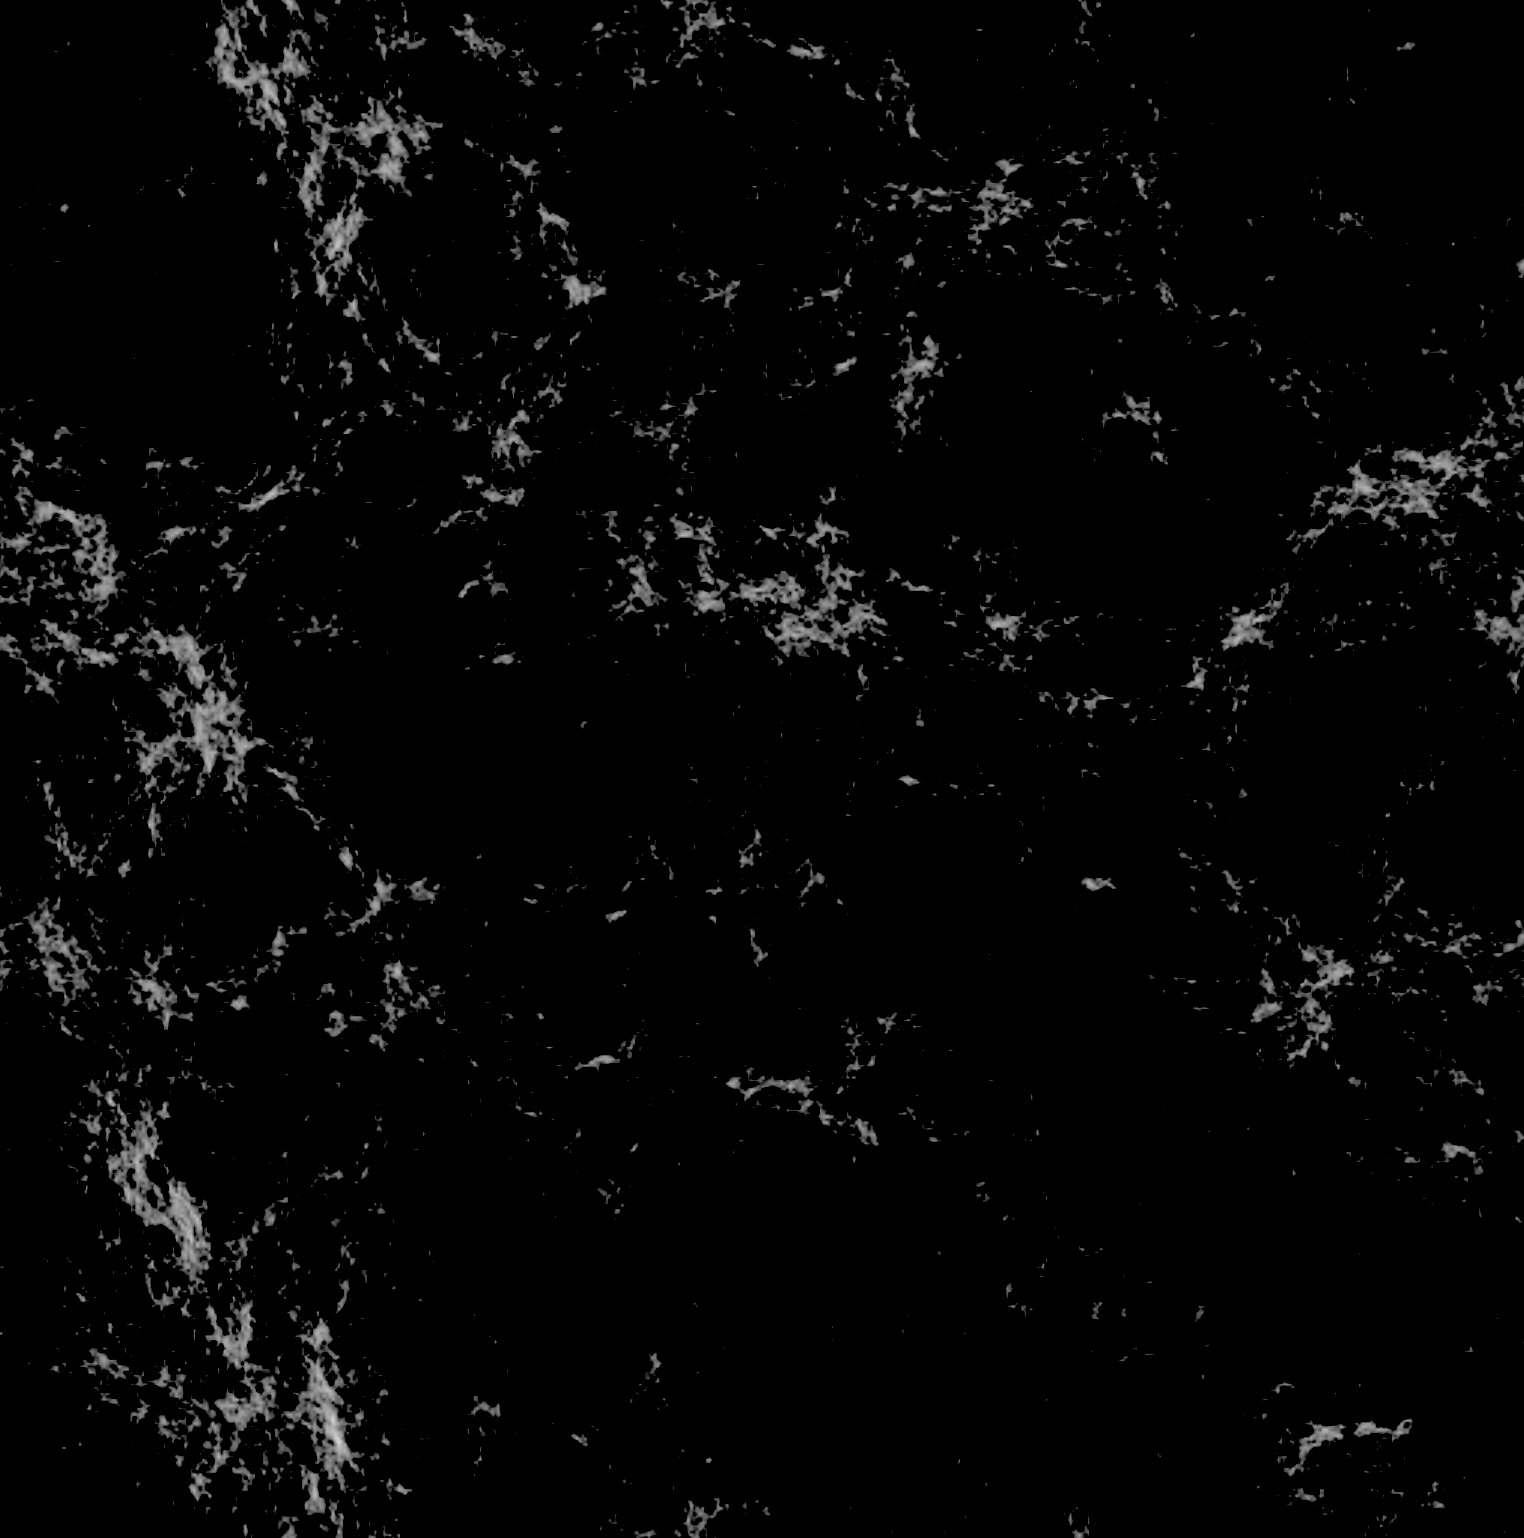
\includegraphics[width=0.40\textwidth]{"images/foam_texture.png"}
    \captionof{figure}{Foam Texture}
    \label{fig:foam_texture}
\end{minipage}

\subsubsection{Foam Accumilation}
Curretlly the foam apears and diasapears quicly, however in real life the foam accumilates and disapears over time.
We can introduce foam accumilation by compering previous and current foam values:
\begin{lstlisting}[caption={Foam Accumilation}, frame=single, numberstyle=\small\color{gray}, captionpos=b]
    float accumulation = 
    LastFoamValue - FoamDecay * DeltaTime / max(currentFoam, 0.5);
    float foam = max(accumulation, currentFoam);
\end{lstlisting}
This results in pleasing foam accumilation:

\begin{minipage}{1\textwidth}
    \centering
    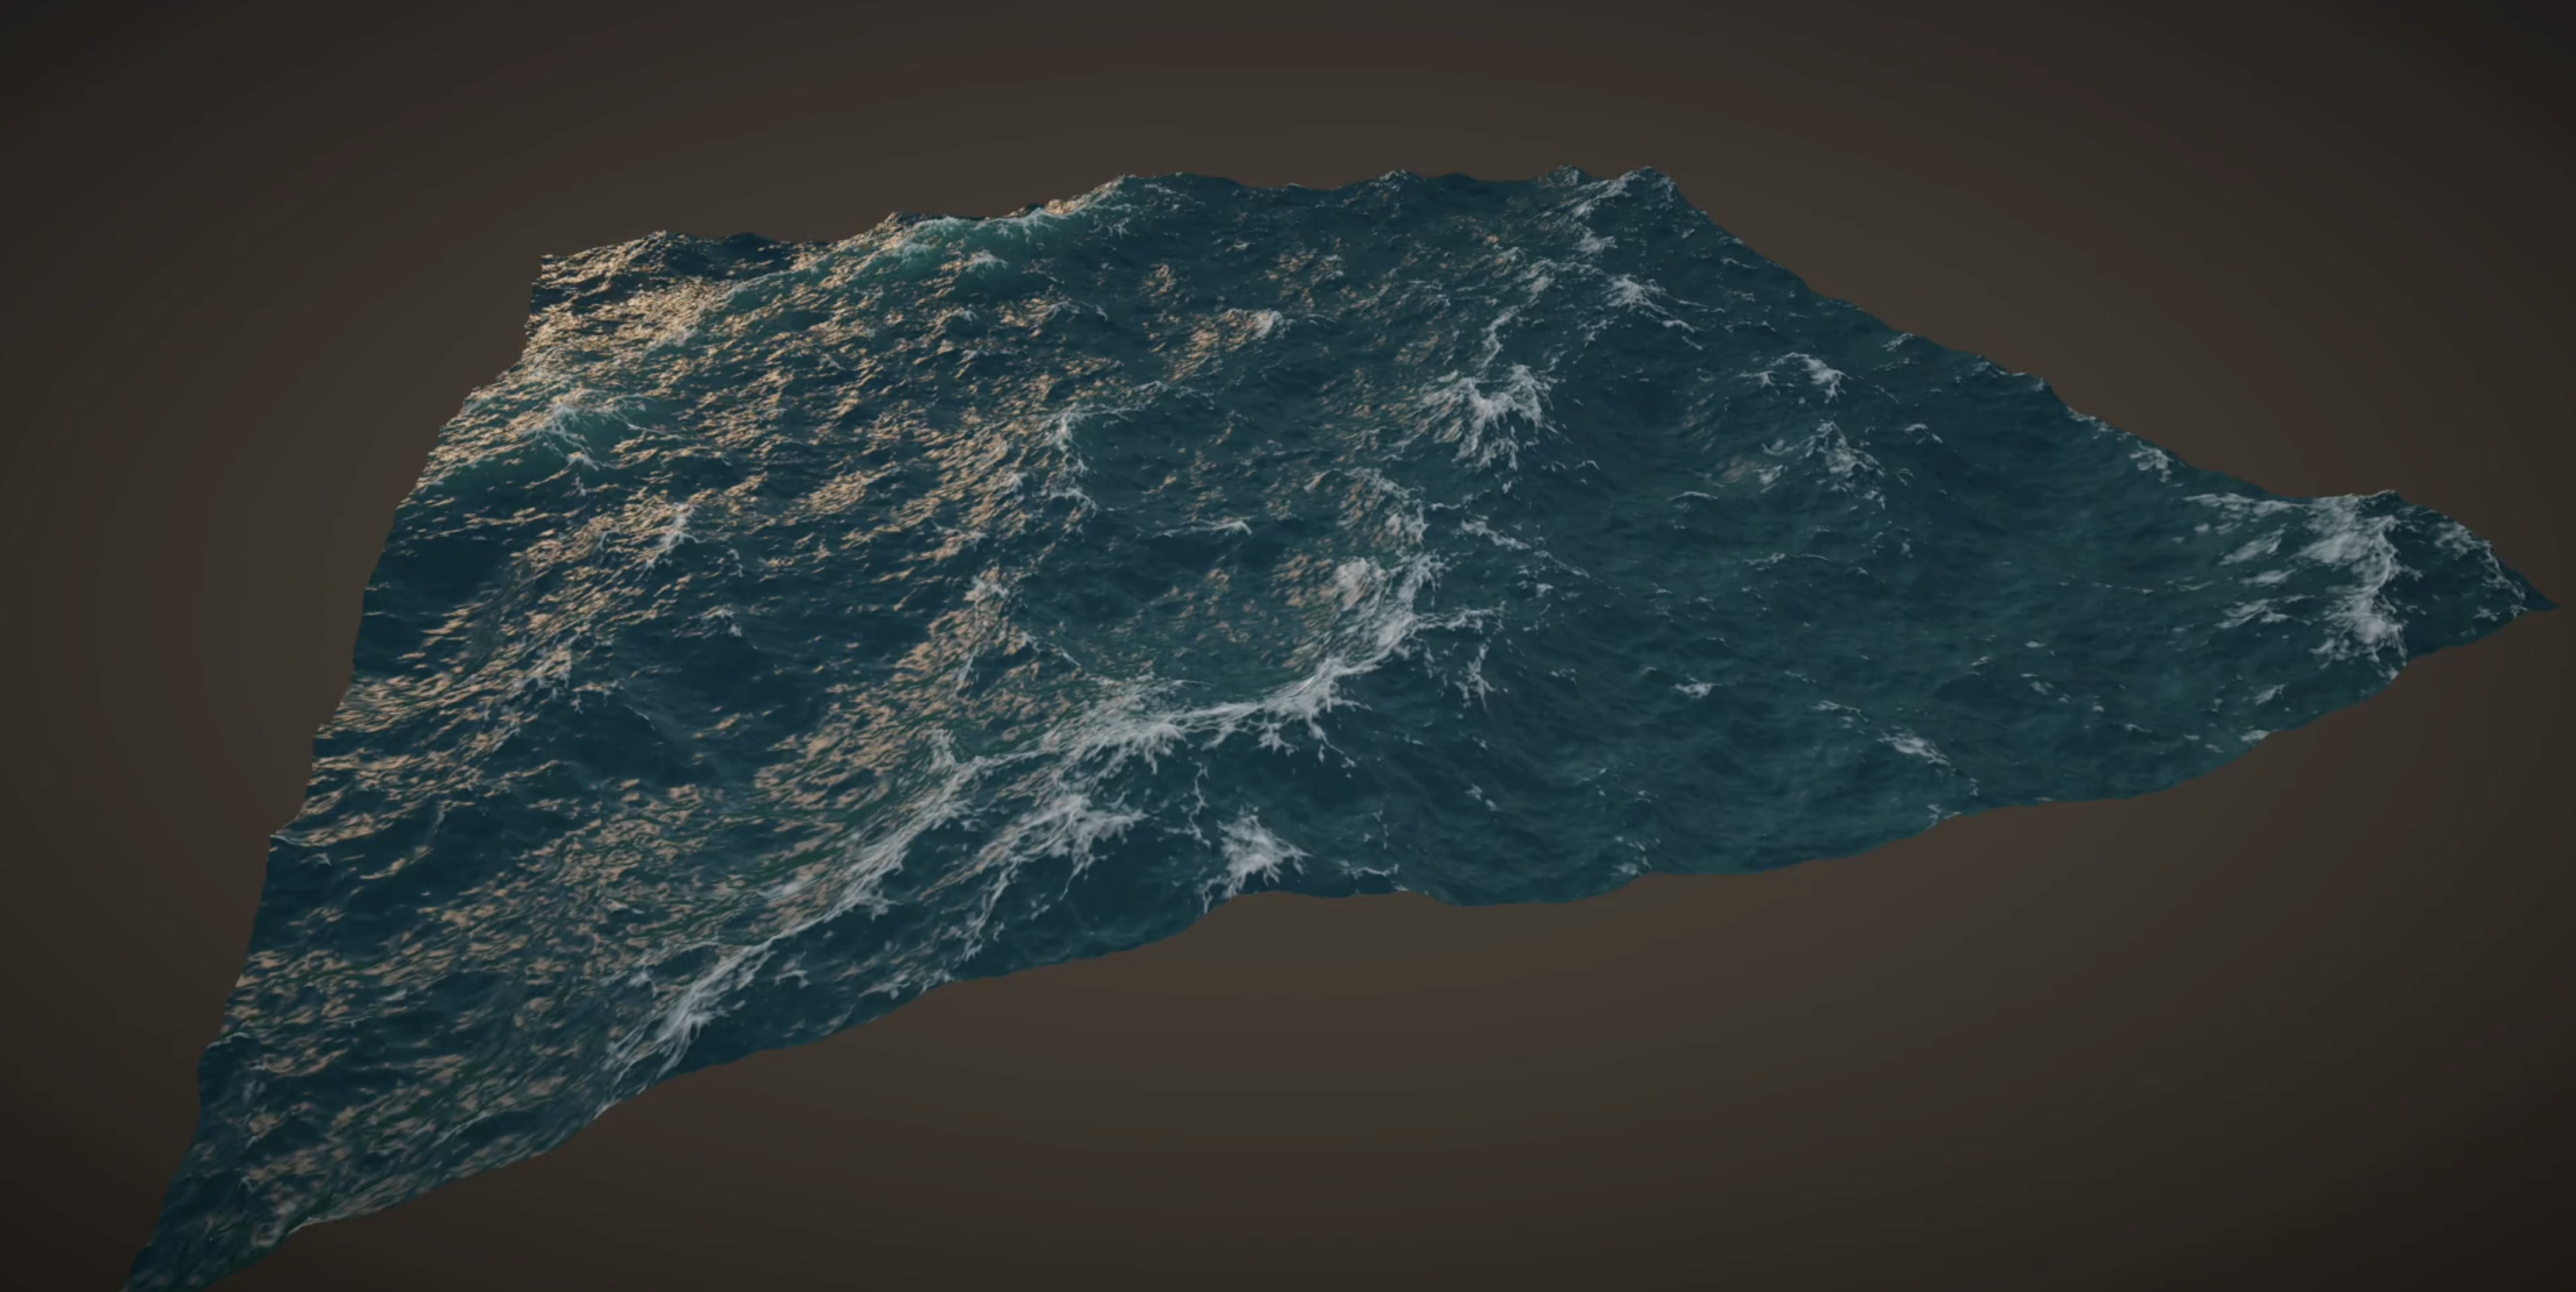
\includegraphics[width=0.8\textwidth]{"images/ocean_with_foam.png"}
    \captionof{figure}{Ocean With Foam}
    \label{fig:ocean_with_foam}
\end{minipage}

\section{Multiple Cascades}
At this stage our ocean with texture 512x512 simulates 262,144 distinc waves however the tilling is still noticible \ref{fig:ocean_with_tilling}.

\begin{minipage}{1\textwidth}
    \centering
    \includegraphics[width=0.8\textwidth]{"images/tilling_ocean.png"}
    \captionof{figure}{Ocean with Tilling, using 512x512 texture}
    \label{fig:ocean_with_tilling}
\end{minipage}

To counter this we could increase our simulation texture however even FFT becomes expensive really fast.
Another approuch is to simulate multiple cascades for diffrent wave lengths $k$ \ref{fig:cascades} and diffrent $l$ length scales. We can split our simulation into 3 parts, big waves, medium waves and small waves.

\begin{minipage}{1\textwidth}
    \centering
    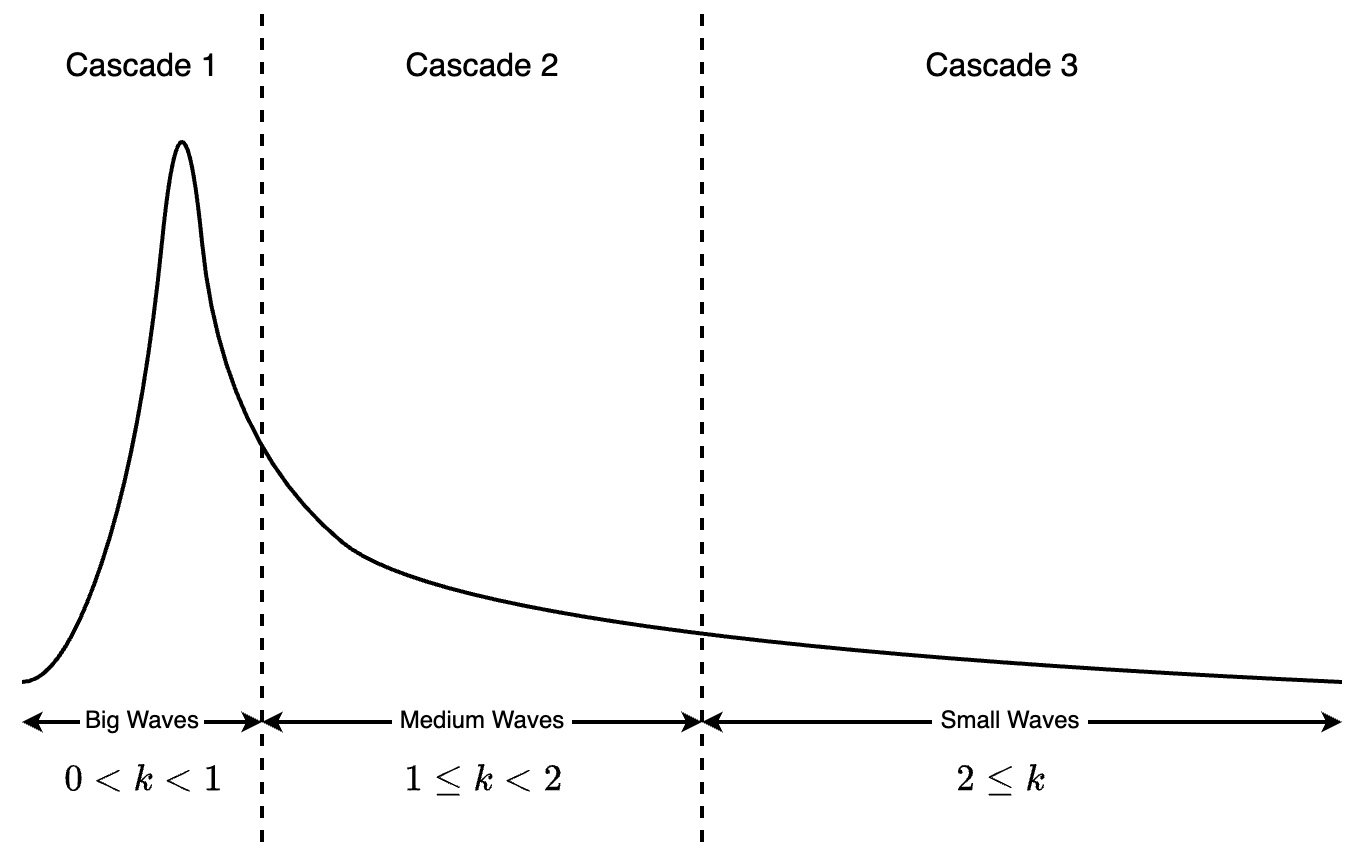
\includegraphics[width=0.8\textwidth]{"images/cascades.png"}
    \captionof{figure}{Cascades}
    \label{fig:cascades}
\end{minipage}
When it comes to chosing $l$ we need to follow these steps:
\begin{enumerate}
    \item We chose bigger $l$ for bigger waves as we are more likly to notice tilling with big waves
    \item We chose smaller $l$ for smaller waves as we are less likly to notice tilling with small waves
\end{enumerate}
This results ocean that has less tilling and more detail \ref{fig:ocean_with_cascades}.
\begin{minipage}{1\textwidth}
    \centering
    \includegraphics[width=0.8\textwidth]{"images/ocean_with_cascades.png"}
    \captionof{figure}{Ocean with Cascades, using 3x(512x512) textures}
    \label{fig:ocean_with_cascades}
\end{minipage}

One of the main pros of having multiple cascades is reduction in performance cost, as we can have similar results of 512x512 with 3x(256x256) xtextures as shown in figure \ref{fig:ocean_with_cascades_256}.

\begin{minipage}{1\textwidth}
    \centering
    \includegraphics[width=0.8\textwidth]{"images/ocean_cascades_256.png"}
    \captionof{figure}{Ocean with Cascades, using 3x(256x256) textures}
    \label{fig:ocean_with_cascades_256}
\end{minipage}

% Before we start, all callculations were taken inside GPU, using HLSL language. This allows us to use parallelism and speed up the process dramatically.
% As FFT requires our sample data length be power of 2, we will use $n \cdot n = 512 \text{x} 512$ textures to represent our data.

% \section{Spectrum Generation}
% \subsection{Tessendorf Spectrum}
% To generate height map \ref{eq:height_map} for our ocean we firstly need to generate spectrum. Firstlly, I chose to use J. Tessendorf's spectrum model \ref{eq:tessendorf_spectrum} as this was straight forward to implement:
% $$
% P_h(\mathbf{k}) = A \frac{e^{-1/(kl)^{2}}}{k^{4}}| \mathbf{\hat{k}} \cdot \mathbf{w} |^{6}
% $$
% where $\mathbf{k} = (k.x, k.y)$, $k.x = 2 * \pi (x.x - n/2)/ l$, $k.y = 2 * \pi (x.y - n/2)/ l$, $l$ is the the length scale of the ocean, 
% anx $\mathbf{x} = (x.x, x.y)$ is current position in the texture. 

% \subsection{TMA Spectrum}
% However, this model was not perfect, as it produced waves that didn't seem to transfer energy in the right way and the waves didn't seem to follow wave dircetion.
% Therefore, I decided to use JONSWAP spectrum with TMA correction that was suggested by \cite{horvath2015} \ref{eq:tma_spectrum}, however in our case $h$ will be constant therefore we can rewrite the function as:
% \begin{equation}
%     S_{TMA}(\omega) = S_{JONSWAP}(\omega) \cdot S_{TMA}(\omega)    
% \end{equation}
% Currentlly, we have two problems with this equation. Firstlly, this spectrum is non-directional, so we need to add directionality to it. Secondly, 
% this spectrum accepts $\omega$ as input, but as we following J. Tessendorf's \cite{tessendorf2001} paper, we need to use $\mathbf{k}$ as input. 

% \subsection{Directional Spectrum}



% According earlier expressed equation \ref{eq:height_map} we use DFT to calculate height map. Because we going to use FFT we can remove the exponential part as this will be calculated inside FFT algorithm:
% \begin{equation}
%     h(\mathbf{x}) = \sum_{\mathbf{k}} \tilde{h}(\mathbf{k}, t)
% \end{equation}
% , we can see that fft-based representation expresses ocean height at horizontal plane $\mathbf{x} = (x, y)$ "as the sum of sinusoids with complex, time-dependent amplitudes"\cite{tessendorf2001}.
% where, $\mathbf{k} = 2\pi $

\justifying
\chapter{Results}
\label{chapter3}

<Results, evaluation (including user evaluation) {\em etc.} should be described in one or more chapters. See the `Results and Discussion' criterion in the mark scheme for the sorts of material that may be included here.>
\section{Performance}

% table for performance
\begin{table}[h]
    \centering
    \begin{tabular}{|c|c|c|}
        \hline
        \textbf{GPU} & \textbf{Texture Size} & \textbf{Time} \\
        \hline
        M1 & 256x256 & 4.97ms \\
        \hline
        M1 & 512x512 & 40.27ms \\
        \hline
        M1 & 1024x1024 & x-code didn't show performance \\
        \hline
    \end{tabular}
\end{table}

[FINISH THIS WHEN RESULTS RETRIEVED FROM UNIVERSITY]

\section{Comparison} 

\subsection{Spectrums}
The main diffrence comes to what kind of spectrum you use for FFT based oceans. The proposed "Phillips" spectrum \ref{fig:phillip_spectrum_comp} by \cite[J. Tessendorf]{tessendorf2001} has issues with energy transformation and following the wind direction. 
The proposed TMA spectrum \ref{fig:tma_spectrum_comp} handles energy transformation way more relistic and does not have any issues following the wind direction. This is mostly because that TMA is based on empirical data.
You can see clear diffrence between "Phillips" spectrum and TMA spectrum:

\begin{minipage}{0.48\textwidth}
    \centering
    
\includegraphics[width=0.8\textwidth]{"images/phillip_spectrum_comp.png"}
    \captionof{figure}{Height Map with $P_h$}
    \label{fig:phillip_spectrum_comp}
\end{minipage}
\hfill
\begin{minipage}{0.48\textwidth}
    \centering
    
\includegraphics[width=0.8\textwidth]{"images/tma_spectrum_comp.png"}
    \captionof{figure}{Height Map using TMA Spectrum}
    \label{fig:tma_spectrum_comp}
\end{minipage}

\subsection{Real world oceans}
When it comes to calm ocean, the FFT based ocean with TMA spectrum performs extremelly well and holds the desired shape as shown in figures \ref{fig:real_calm_ocean} and \ref{fig:fake_calm_ocean}.
\begin{table}[h]
    \centering
    \begin{tabular}{|c|c|c|c|c|c|c|c|c|c|}
        \hline
        \textbf{Spectrum} & \textbf{Size} & $\mathbf{l_1}$ & $\mathbf{l_2}$ & $\mathbf{l_3}$ & $\mathbf{\lambda}$ & $\mathbf{U_{10}}$ & \textbf{Fetch} & \textbf{Depth} \\
        \hline
        256x256 & TMA & 256 & 100 & 10 & 0.9 & 0.02 m/s & 1000 km & 500 m \\
        \hline
    \end{tabular}
    \caption{Calm Ocean Parameters}
    \label{tab:calm_ocean}
\end{table}

\begin{minipage}{0.48\textwidth}
    \centering
    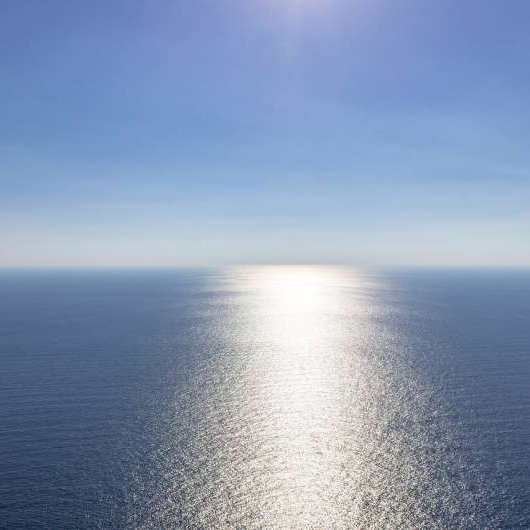
\includegraphics[width=0.8\textwidth]{"images/real_calm_ocean.jpg"}
    \captionsetup{justification=centering}
    \captionof{figure}{Calm Atlantic Ocean\\ Credits: CC0 Public Domain}
    \label{fig:real_calm_ocean}
\end{minipage}
\hfill
\begin{minipage}{0.48\textwidth}
    \centering
    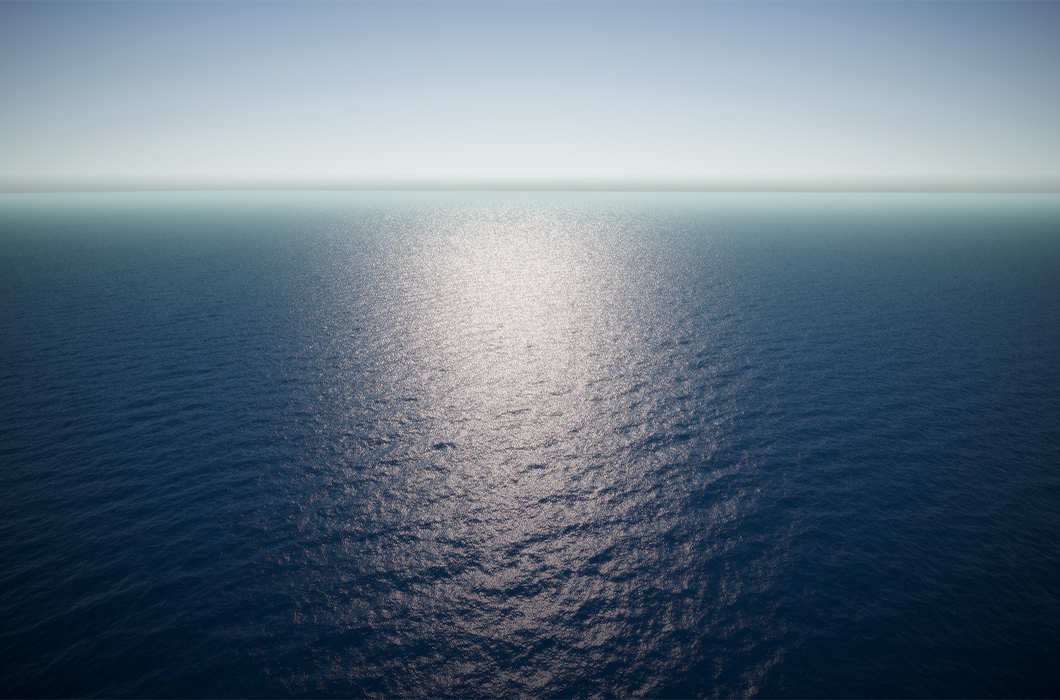
\includegraphics[width=0.8\textwidth]{"images/fake_calm_ocean.png"}
    \captionof{figure}{FFT Calm Ocean}
    \label{fig:fake_calm_ocean}
\end{minipage}

When it comes to stormy ocean where huge waves is expected the general shape of an ocean is still relistic
and can hadle the big waves without any trouble, and because of diffrent cascades the tilling is bearlly noticible as shown in the following figures \ref{fig:real_stormy_ocean} and \ref{fig:fake_stormy_ocean}.
\begin{table}[h]
    \centering
    \begin{tabular}{|c|c|c|c|c|c|c|c|c|c|}
        \hline
        \textbf{Spectrum} & \textbf{Size} & $\mathbf{l_1}$ & $\mathbf{l_2}$ & $\mathbf{l_3}$ & $\mathbf{\lambda}$ & $\mathbf{U_{10}}$ & \textbf{Fetch} & \textbf{Depth} \\
        \hline
        256x256 & TMA & 700 & 256 & 70 & 0.9 & 21 m/s & 1000 km & 500 m \\
        \hline
    \end{tabular}
    \caption{Stormy Ocean Parameters}
    \label{tab:stormy_ocean}
\end{table}
where each $l$ is the wave length scale of each cascade.

\begin{minipage}{0.48\textwidth}
    \centering
    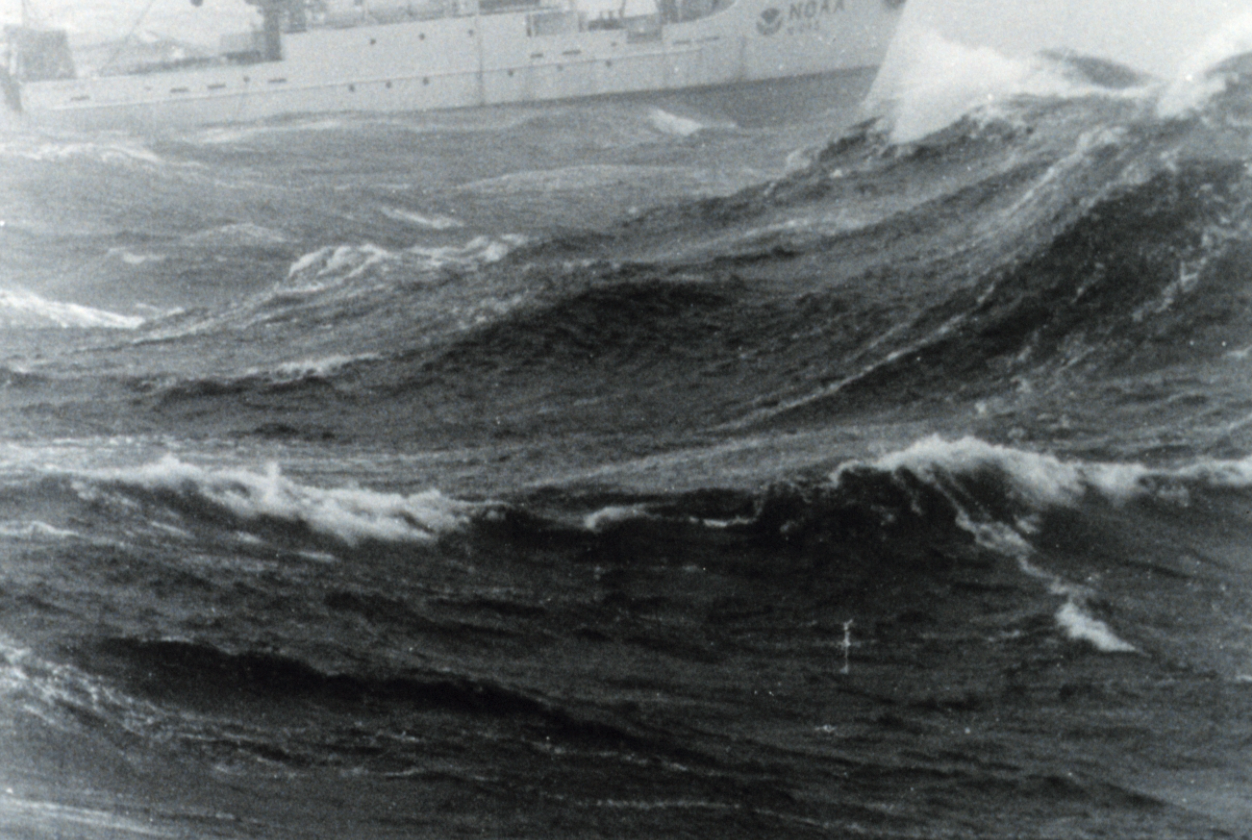
\includegraphics[width=0.8\textwidth]{"images/real_stormy_ocean.png"}
    \captionsetup{justification=centering}
    \captionof{figure}{Calm Atlantic Ocean\\ Credits: CC0 Public Domain}
    \label{fig:real_stormy_ocean}
\end{minipage}
\hfill
\begin{minipage}{0.48\textwidth}
    \centering
    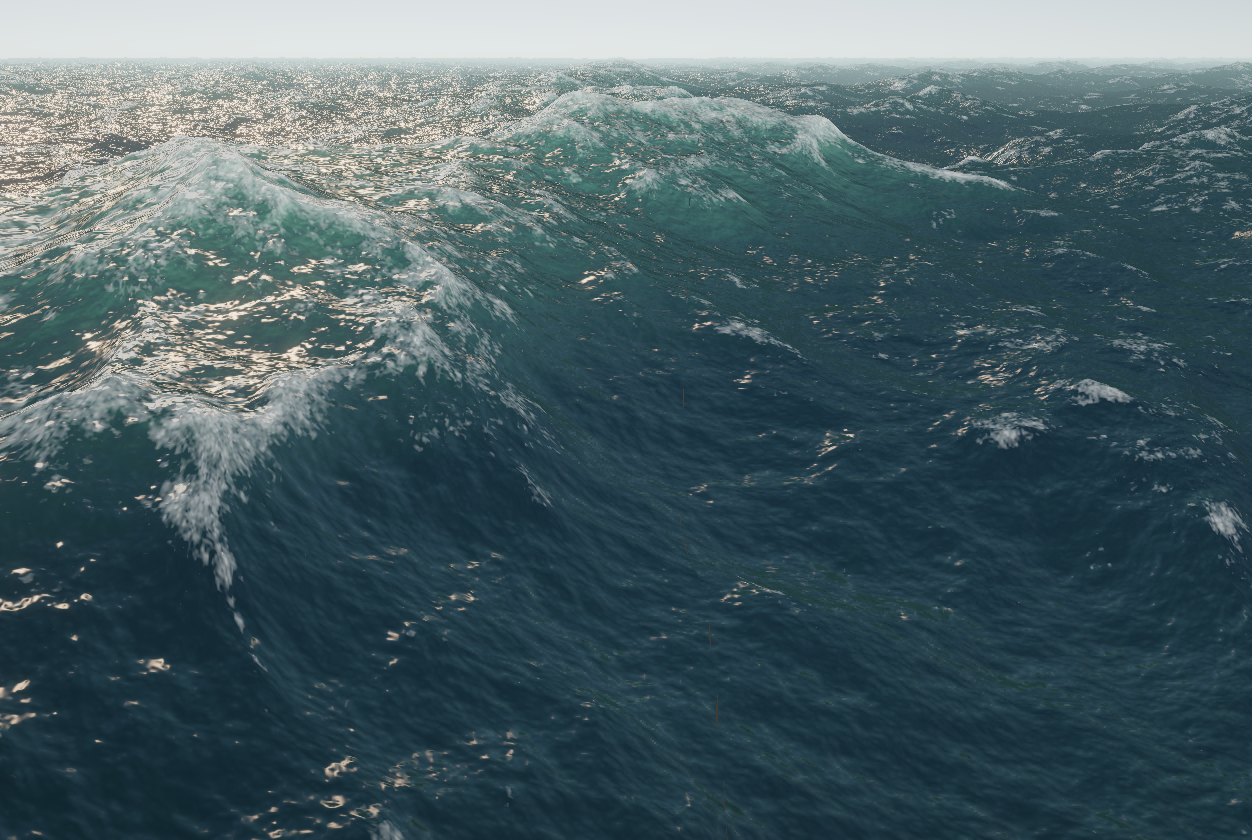
\includegraphics[width=0.8\textwidth]{"images/fake_stormy_ocean.png"}
    \captionof{figure}{Height Map using\\ TMA Spectrum}
    \label{fig:fake_stormy_ocean}
\end{minipage}

\section{Diffrent Outputs}

\section{Known Problems}
\chapter{Discussion}
\label{chapter4}

<Everything that comes under the `Results and Discussion' criterion in the mark scheme that has not been addressed in an earlier chapter should be included in this final chapter. The following section headings are suggestions only.>

\section{Conclusions}

FFT ocean are fast and produces relistic enought oceans.\\
Having FFT algorithm is crucial and DFT wouldn't be sufficient.\\
The key of making good ocean is having spectrum that is based on empirical data.\\
To remove tiling instead of making bigger texture simulation we can simulate diffrent cascades and overlap them thus having more detail and more performance and less tilling\\
We use modified Phong Shader, however we should switch to PBR as this would give us more relistic results.


\section{Ideas for future work}
Interactive Water\\
PBR Shading\\
Buoyancy\\
Foam Spray\\
This technique produces realistic oceans in a cost-efficient way suitable for real-time rendering. However, it does not support interactive waves. For that, J. Tessendorf proposed a method called “iWaves” \cite{tessendorf2004} and a later upgraded version “eWaves” \cite{tessendorf2014}.




% Adds references to the table of contents.
\addcontentsline{toc}{chapter}{References}

% All your bibtex entries should go in the file called "refs.bib".
\bibliography{refs}

% All appendices you have go in a file called "appendices.tex".
\begin{appendices}

%
% The first appendix must be "Self-appraisal".
%
\chapter{Self-appraisal}

\section{Critical self-evaluation}

In the initial stages, a comprehensive evaluation of multiple libraries was conducted to select the most suitable one for our project. This selection process was underpinned by a thorough understanding of the theoretical aspects of FFT waves, which we developed by reviewing numerous research papers. To further solidify our foundational knowledge, we created a naive sum of sins project to understand the basics of ocean generation.

With a detailed workflow and a graphed algorithm in place, we embarked on the project, ensuring that unnecessary refactoring was minimized and adherence to the project timeline was maintained. The project was initially implemented in a simplistic manner to grasp the underlying theory. Once a solid understanding was established, the project was advanced to a more complex level to optimize computational efficiency. Throughout this process, data visualization was employed at every step to ensure the absence of bugs and validate the accuracy of our results.

Upon completion of the project, the results produced were compared with real-world data. This comparison confirmed the realism of the ocean generated by our project, attesting to the success of our approach. Thus, the project execution demonstrated a high degree of planning, theoretical understanding, practical implementation, and validation, resulting in a realistic and efficient ocean generation technique.

\section{Personal reflection and lessons learned}

This project served as a comprehensive learning experience, enhancing our technical skills, academic research abilities, professional communication, and project management strategies. We learned the importance of clear and timely communication, particularly with superiors, when the project was initially undertaken in Unity without prior approval. This oversight was later rectified by submitting a detailed request analyzing different approaches.

The project also provided an opportunity to delve into academic research, enhancing our ability to effectively search for and read research papers. On the technical front, we gained experience in using compute shaders and expressing complex mathematical equations, which was instrumental in creating the FFT algorithm and generating a realistic ocean.

Additionally, the project honed our report writing skills and reinforced the necessity of obtaining necessary permissions before embarking on significant project decisions.

\section{Legal, social, ethical and professional issues}

\subsection{Legal issues}
In the context of this project, the primary legal considerations pertain to the use of Unity, a third-party tool. As the entirety of the codebase was authored independently, there are no concerns regarding the infringement of external code licenses. However, it is crucial to adhere to the terms and conditions stipulated by Unity’s license agreement. This adherence ensures the lawful utilization of Unity’s resources and capabilities, thereby aligning the project with the requisite legal standards.

\subsection{Social issues}
The potential applications of this project, particularly in domains such as video games or cinematic productions, could have notable social implications. Specifically, the manner in which the ocean is represented and rendered using this implementation could influence societal perceptions of marine environments. As such, it is crucial to ensure that the oceanic simulations generated are as accurate and realistic as possible, to foster an authentic understanding and appreciation of our oceans.

\subsection{Ethical issues}
In the realm of ethical considerations, it is imperative to ensure that the ocean simulation does not misrepresent or oversimplify the inherently complex marine phenomena. Such misrepresentations could potentially lead to misunderstandings or misuse of the work, thereby violating ethical guidelines of accuracy and truthfulness in scientific representation.

Furthermore, the consideration of making this project open-source aligns with the ethical principle of knowledge sharing in the academic and scientific community. By doing so, the project could serve as a learning resource for others, promoting transparency, collaboration, and collective learning.

\subsection{Professional issues}
A key professional consideration in this project is the adherence to industry standards and best practices in coding and documentation. This adherence ensures the maintainability, readability, and scalability of the code, thereby enhancing its longevity and usability.

Furthermore, it is crucial to stay abreast of the latest advancements in the field. This includes keeping up-to-date with new versions or features of Unity, advancements in FFT algorithms, or GPU programming techniques. Such continual learning and adaptation are essential for maintaining the relevance and effectiveness of our work in a rapidly evolving field.
%
% Any other appendices you wish to use should come after "Self-appraisal". You can have as many appendices as you like.
%
\chapter{External Material}
%<This appendix should provide a brief record of materials used in the solution that are not the student's own work. Such materials might be pieces of codes made available from a research group/company or from the internet, datasets prepared by external users or any preliminary materials/drafts/notes provided by a supervisor. It should be clear what was used as ready-made components and what was developed as part of the project. This appendix should be included even if no external materials were used, in which case a statement to that effect is all that is required.>
\section{Skyboxes}
Additional skyboxes utilized in this project were procured from the Unity Asset Store. The specific asset employed is freely available and grants comprehensive permissions for unrestricted usage. This approach aligns with the principles of ethical use of third-party resources in academic projects. The asset can be accessed at the following URL: \url{https://assetstore.unity.com/packages/2d/textures-materials/sky/skybox-series-free-103633}.

%
% Other appendices can be added here following the same pattern as above.
%
\chapter{Additional Results}
The outcomes of the conducted experiments, encapsulated in video format, are accessible in the designated \href{https://github.com/uol-feps-soc-comp3931-2324-classroom/final-year-project-Biebras}{Git repository}.

\end{appendices}


\end{document}

